\section{Parameter Estimates}
\label{sec:result_paramEst}

\begin{figure}[htbp]
  \centering
  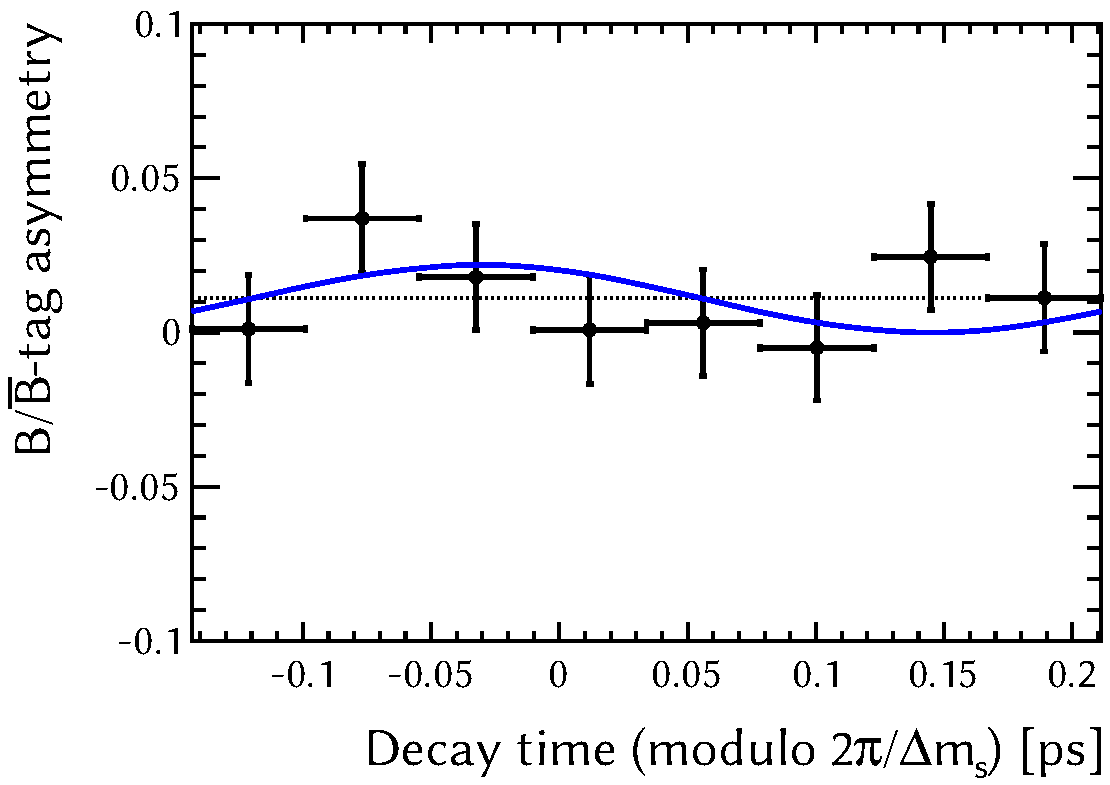
\includegraphics[width=0.75\textwidth]{graphics/results/asym}
  \caption{Background-subtracted asymmetry in the numbers of decay candidates with $\Bs$ and $\Bsbar$ flavour tags (data points)
           and the corresponding asymmetry in the PDF (blue line) as a function of decay time.
           Data from the full decay-time range are mapped onto one period of the expected oscillation in the asymmetry.
           Decay candidates are weighted by the product of the corresponding estimated dilution factors from decay-time resolution
           and wrong tags to optimize the significance of the displayed asymmetry.}
  \label{fig:BBbarAsymmetry}
\end{figure}

\begin{figure}[tbp]
  \centering
  \begin{subfigure}{0.49\textwidth}
    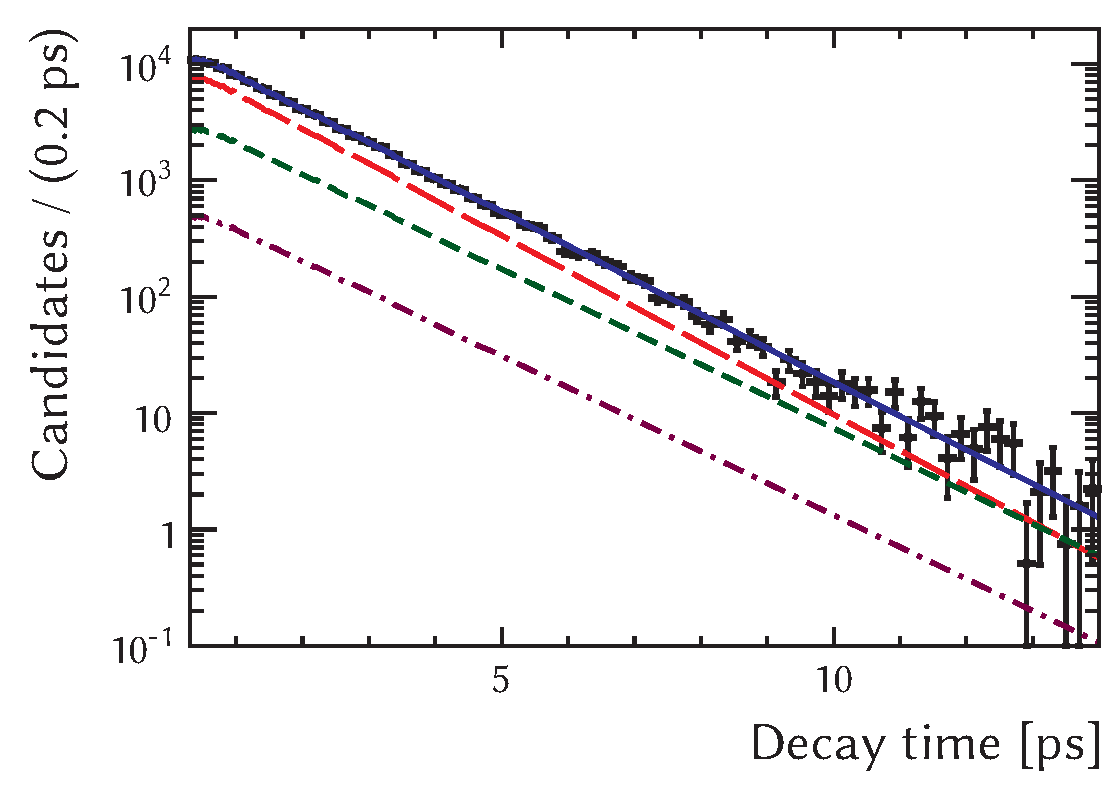
\includegraphics[width=\textwidth]{graphics/results/timeLog}
    \caption{}
  \end{subfigure}
  \hfill%
  \begin{subfigure}{0.49\textwidth}
    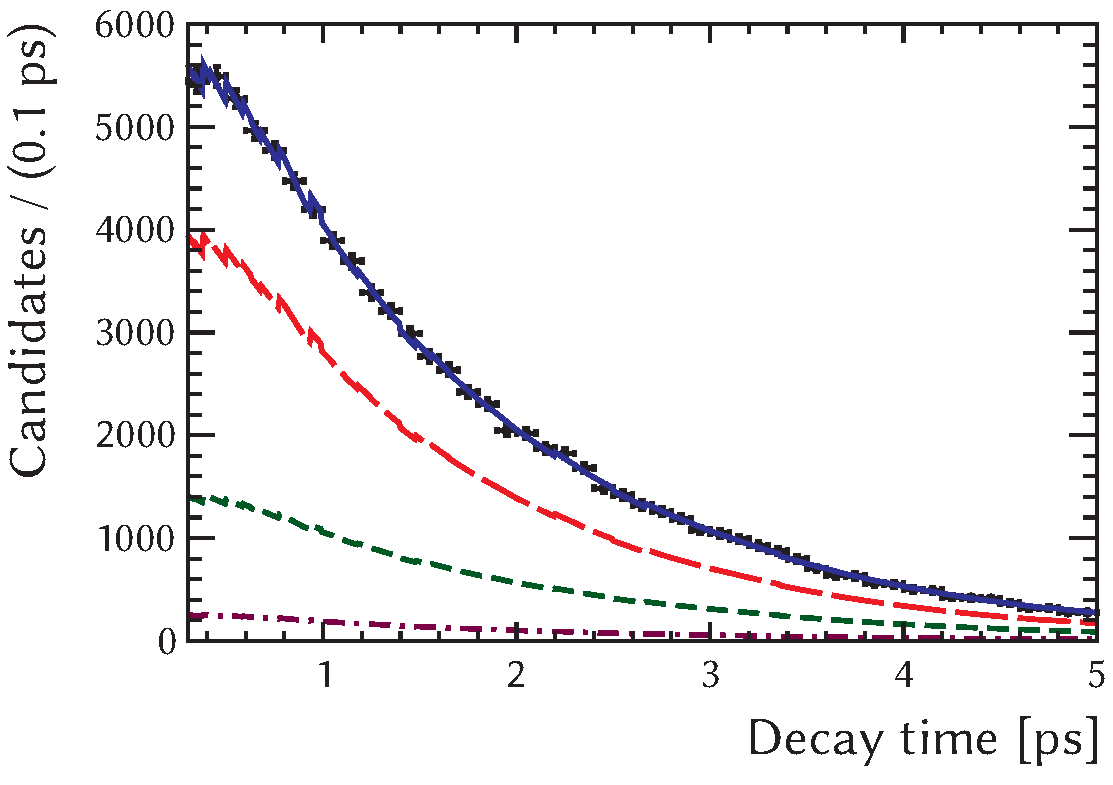
\includegraphics[width=\textwidth]{graphics/results/timeLin}
    \caption{}
  \end{subfigure}

  \caption{Background-subtracted distribution of decay candidates in decay time (data points)
           and the corresponding one-dimensional projection of the PDF (blue line).
           Figure~(a) shows the distribution in the full range between 0.3 and 14\unitsp{}ps
           on a logarithmic vertical scale, while Figure~(b) shows the distribution between 0.3 and 5\unitsp{}ps
           on a linear vertical scale.
           Additional PDF projections are shown for the CP-even (long-dashed, red line) and CP-odd (short-dashed, green line)
           components of \BstoJpsiphi{} and for the S-wave (dashed-dotted, magenta line).}
  \label{fig:timeProjections}
\end{figure}

\begin{figure}[tbp]
  \centering
  \begin{subfigure}{0.49\textwidth}
    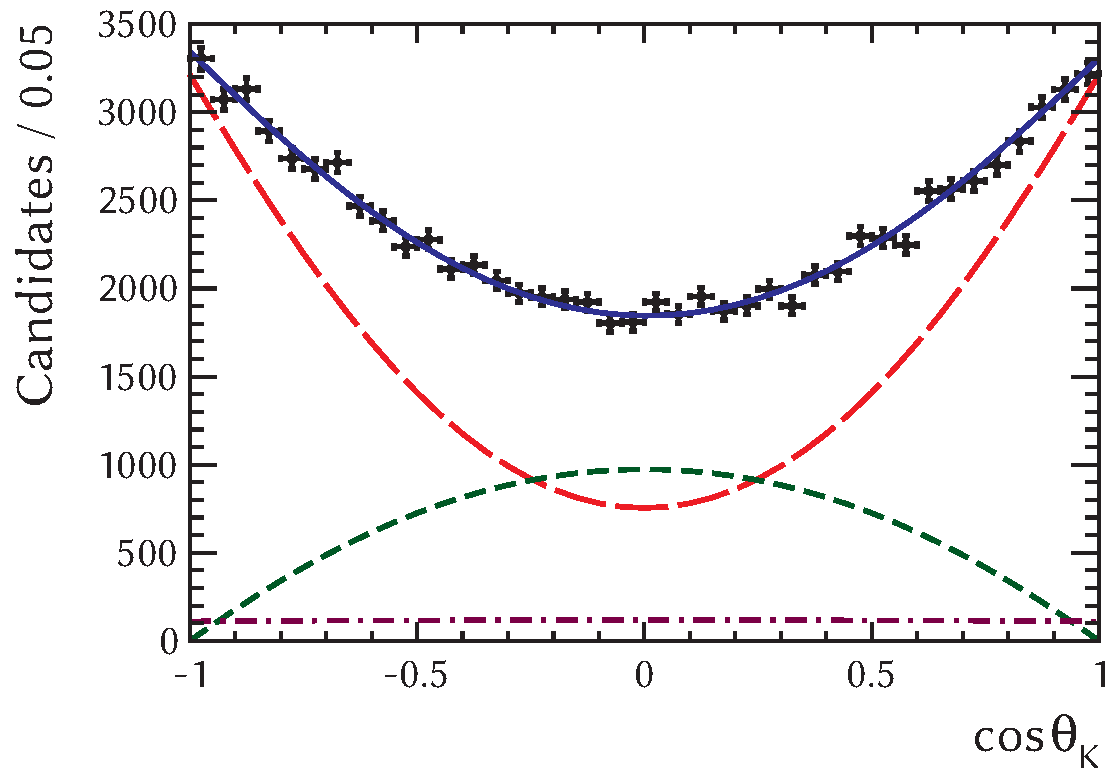
\includegraphics[width=\textwidth]{graphics/results/ctk}
    \caption{}
  \end{subfigure}
  \hfill%
  \begin{subfigure}{0.49\textwidth}
    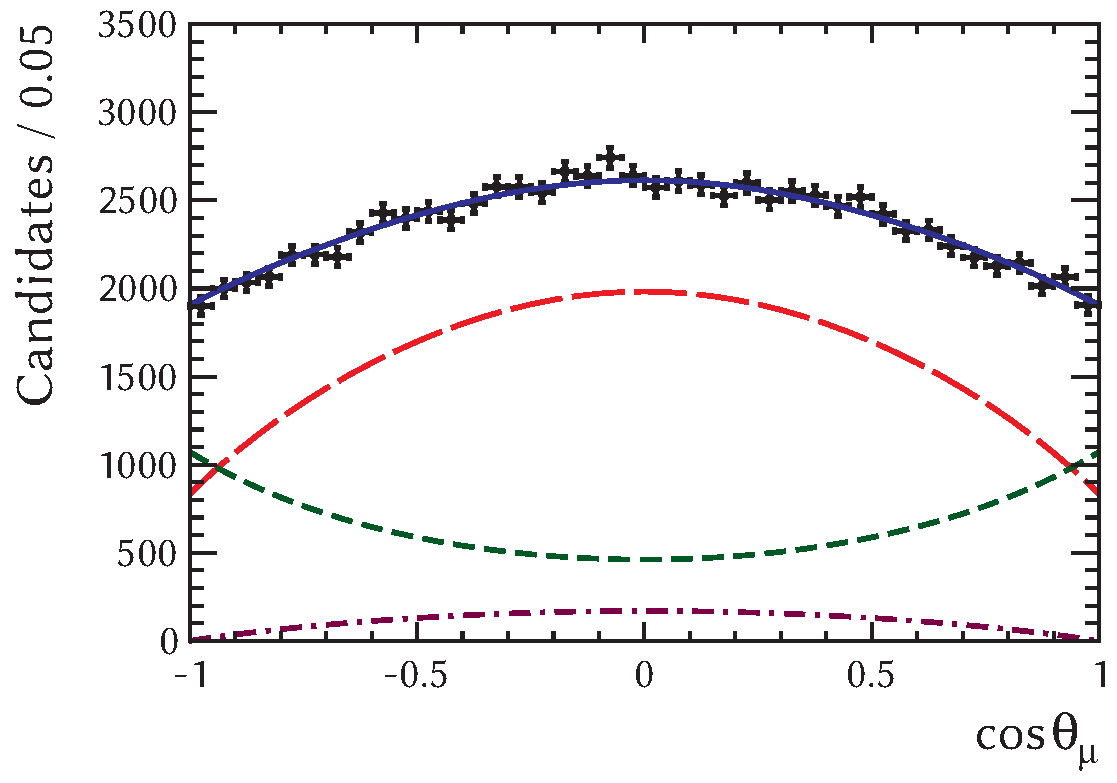
\includegraphics[width=\textwidth]{graphics/results/ctl}
    \caption{}
  \end{subfigure}

  \vspace*{0.02\textwidth}
  \begin{subfigure}{0.49\textwidth}
    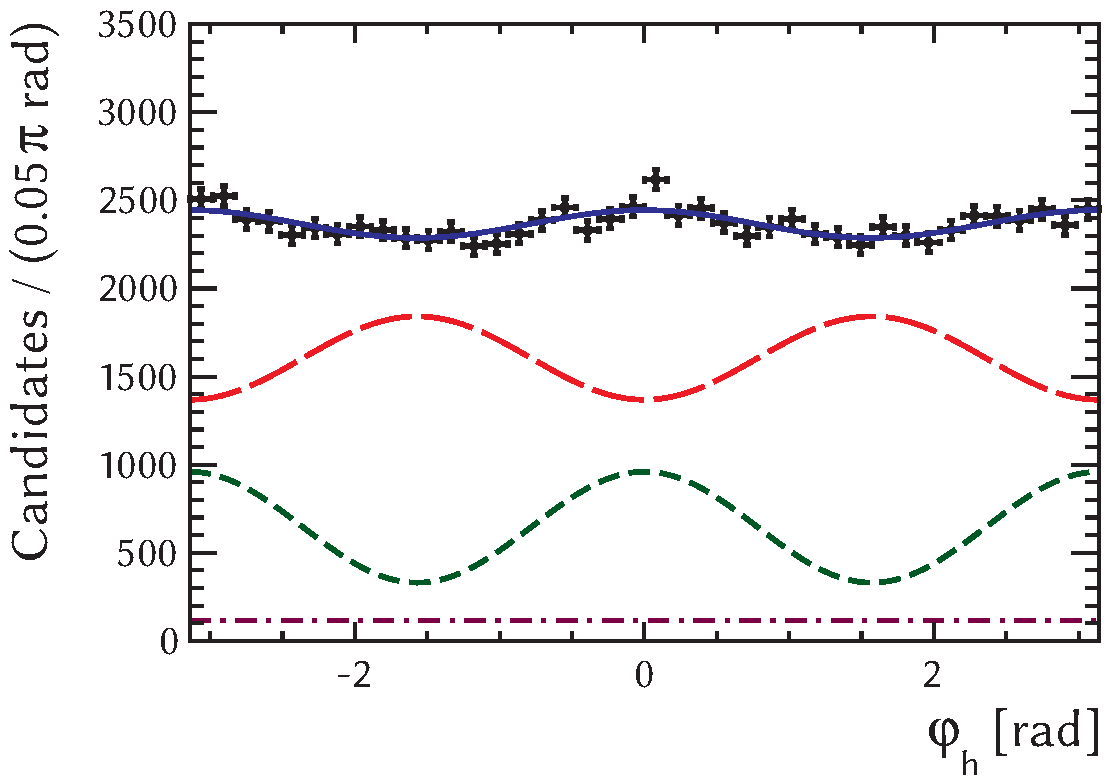
\includegraphics[width=\textwidth]{graphics/results/phi}
    \caption{}
  \end{subfigure}

  \caption{Background-subtracted distribution of decay candidates in decay angles (data points)
           and the corresponding one-dimensional projections of the PDF (blue line).
           The distributions of $\cthetaK$, $\cthetal$, and $\phihel$ are shown in Figures~(a), (b), and (c), respectively.
           Additional PDF projections are shown for the CP-even (long-dashed, red line) and CP-odd (short-dashed, green line)
           components of \BstoJpsiphi{} and for the S-wave (dashed-dotted, magenta line).}
  \label{fig:angleProjections}
\end{figure}

\begin{table}[htbp]
  \centering
  \caption{}
  \label{tab:result_paramEst_nominal_phi}
  \begin{tabular}{lllcc}
    \hline
    parameter  &  estimate &  uncertainty  &  \multicolumn{1}{l}{pull mean}  &  \multicolumn{1}{l}{pull width}  \\
    \hline
    $\phis$         &  \tm0.06            &  0.05         &  \tm0.018\textpm0.010  &  0.973\textpm0.007  \\
    \hline
    $\Gs$           &  \phantom{+}0.6591  &  0.0033       &    +0.018\textpm0.010  &  0.995\textpm0.007  \\
    $\DGs$          &   +0.079            &  0.009        &    +0.006\textpm0.010  &  0.991\textpm0.007  \\
    $\Dms$          &  \phantom{+}17.70   &  0.06         &  \tm0.011\textpm0.010  &  1.025\textpm0.008  \\
    \hline
    $\magzeroSq$    &  \phantom{+}0.5236  &  0.0034       &    +0.005\textpm0.010  &  1.012\textpm0.007  \\
    $\magperpSq$    &  \phantom{+}0.251   &  0.005        &  \tm0.102\textpm0.010  &  0.997\textpm0.007  \\
    $\FS[1]$        &  \phantom{+}0.43    &  0.05             &  --  &  --  \\
    $\FS[2]$        &  \phantom{+}0.059   &  0.018            &  --  &  --  \\
    $\FS[3]$        &  \phantom{+}0.010   &  +0.007 \tm0.006  &  --  &  --  \\
    $\FS[4]$        &  \phantom{+}0.008   &  +0.006 \tm0.005  &  --  &  --  \\
    $\FS[5]$        &  \phantom{+}0.045   &  0.016            &  --  &  --  \\
    $\FS[6]$        &  \phantom{+}0.192   &  0.025            &  --  &  --  \\
    \hline
    $\delparzero$   &   +3.26             &  +0.10 \tm0.18  &  \tm0.004\textpm0.013  &  1.261\textpm0.013  \\
    $\delperpzero$  &   +3.04             &  +0.16 \tm0.17  &  \tm0.026\textpm0.011  &  1.058\textpm0.008  \\
    $\delSperp[1]$  &   \multicolumn{2}{l}{%$[\text{+0.65},   \text{+1.07}]$;
                                           %$[\text{+0.5},   \text{+1.4}]$;
                                           $[\text{+0.3},   \text{+2.6}]$}    &  --  &  --  \\
    $\delSperp[2]$  &   \multicolumn{2}{l}{%$[\text{+1.59},   \text{+2.38}]$;
                                           %$[\text{+0.7},   \text{+2.5}]$;
                                           $[\text{+0.5},   \text{+2.7}]$}    &  --  &  --  \\
    $\delSperp[3]$  &   \multicolumn{2}{l}{%$[\text{+0.30},   \text{+0.86}]$;
                                           %$[\text{+0.2},   \text{+2.1}]$;
                                           $[\text{+0.1},   \text{+2.8}]$}    &  --  &  --  \\
    $\delSperp[4]$  &   \multicolumn{2}{l}{%$[\text{\tm0.71}, \text{\tm0.23}]$;
                                           %$[\text{\tm1.5}, \text{\tm0.1}]$;
                                           $[\text{\tm2.6}, \text{+0.1}]$}    &  --  &  --  \\
    $\delSperp[5]$  &   \multicolumn{2}{l}{%$[\text{\tm0.85}, \text{\tm0.47}]$;
                                           %$[\text{\tm2.7}, \text{\tm0.4}]$;
                                           $[\text{\tm2.8}, \text{\tm0.2}]$}  &  --  &  --  \\
    $\delSperp[6]$  &   \multicolumn{2}{l}{%$[\text{\tm1.06}, \text{\tm0.77}]$;
                                           %$[\text{\tm1.3}, \text{\tm0.7}]$;
                                           $[\text{\tm1.6}, \text{\tm0.6}]$}  &  --  &  --  \\
    \hline
  \end{tabular}
\end{table}

\begin{table}[htbp]
  \centering
  \caption{}
  \label{tab:result_paramEst_nominal_lamb_phi}
  \begin{tabular}{lllcc}
    \hline
    parameter  &  estimate &  uncertainty  &  \multicolumn{1}{l}{pull mean}  &  \multicolumn{1}{l}{pull width}  \\
    \hline
    $\phis$         &  \tm0.06            &  0.05     &    +0.008\textpm0.010  &  0.980\textpm0.007  \\
    $\lamsAbs$      &  \phantom{+}0.963   &  0.019    &  \tm0.096\textpm0.011  &  1.052\textpm0.007  \\
    \hline
    $\Gs$           &  \phantom{+}0.6592  &  0.0033   &    +0.026\textpm0.010  &  0.990\textpm0.007  \\
    $\DGs$          &   +0.079            &  0.009    &    +0.014\textpm0.010  &  0.991\textpm0.007  \\
    $\Dms$          &  \phantom{+}17.72   &  0.06     &    +0.009\textpm0.010  &  1.020\textpm0.007  \\
    \hline
    $\magzeroSq$    &  \phantom{+}0.5237  &  0.0034   &  \tm0.002\textpm0.010  &  1.012\textpm0.007  \\
    $\magperpSq$    &  \phantom{+}0.251   &  0.005    &  \tm0.112\textpm0.010  &  1.015\textpm0.007  \\
    $\FS[1]$        &  \phantom{+}0.426   &  0.05             &  --  &  --  \\
    $\FS[2]$        &  \phantom{+}0.059   &  0.018            &  --  &  --  \\
    $\FS[3]$        &  \phantom{+}0.010   &  +0.007 \tm0.006  &  --  &  --  \\
    $\FS[4]$        &  \phantom{+}0.009   &  +0.006 \tm0.005  &  --  &  --  \\
    $\FS[5]$        &  \phantom{+}0.048   &  0.015            &  --  &  --  \\
    $\FS[6]$        &  \phantom{+}0.192   &  0.025            &  --  &  --  \\
    \hline
    $\delparzero$   &   +3.26             &  +0.10 \tm0.17  &    +0.017\textpm0.013  &  1.264\textpm0.014  \\
    $\delperpzero$  &   +3.10             &  +0.14 \tm0.15  &    +0.001\textpm0.011  &  1.075\textpm0.008  \\
    $\delSperp[1]$  &   \multicolumn{2}{l}{%$[\text{+0.66},   \text{+1.07}]$;
                                           %$[\text{+0.5},   \text{+1.4}]$;
                                           $[\text{+0.3},   \text{+2.6}]$}    &  --  &  --  \\
    $\delSperp[2]$  &   \multicolumn{2}{l}{%$[\text{+1.69},   \text{+2.37}]$;
                                           %$[\text{+0.8},   \text{+2.5}]$;
                                           $[\text{+0.6},   \text{+2.7}]$}    &  --  &  --  \\
    $\delSperp[3]$  &   \multicolumn{2}{l}{%$[\text{+0.31},   \text{+0.83}]$;
                                           %$[\text{+0.2},   \text{+1.8}]$;
                                           $[\text{+0.1},   \text{+2.7}]$}    &  --  &  --  \\
    $\delSperp[4]$  &   \multicolumn{2}{l}{%$[\text{\tm0.60}, \text{\tm0.21}]$;
                                           %$[\text{\tm1.1}, \text{\tm0.1}]$;
                                           $[\text{\tm2.3}, \text{+0.1}]$}    &  --  &  --  \\
    $\delSperp[5]$  &   \multicolumn{2}{l}{%$[\text{\tm0.78}, \text{\tm0.46}]$;
                                           %$[\text{\tm1.2}, \text{\tm0.3}]$;
                                           $[\text{\tm2.7}, \text{\tm0.2}]$}  &  --  &  --  \\
    $\delSperp[6]$  &   \multicolumn{2}{l}{%$[\text{\tm1.06}, \text{\tm0.78}]$;
                                           %$[\text{\tm1.3}, \text{\tm0.7}]$;
                                           $[\text{\tm1.6}, \text{\tm0.6}]$}  &  --  &  --  \\
    \hline
  \end{tabular}
\end{table}

\begin{table}[htbp]
  \centering
  \caption{}
  \label{tab:result_paramEst_nominal_polarDep}
  \begin{tabular}{lllcc}
    \hline
    parameter  &  estimate &  uncertainty  &  \multicolumn{1}{l}{pull mean}  &  \multicolumn{1}{l}{pull width}  \\
    \hline
    $\phisav$       &  \tm0.05            &  0.05    &  \tm0.013\textpm0.010  &  0.970\textpm0.007  \\
    $\Delphispara$  &  \tm0.02            &  0.04    &  \tm0.013\textpm0.009  &  0.915\textpm0.006  \\
    $\Delphisperpp$ &  \tm0.003           &  0.029   &    +0.008\textpm0.009  &  0.875\textpm0.006  \\
    $\DelphisS$     &   +0.01             &  0.06    &    +0.164\textpm0.011  &  0.959\textpm0.006  \\
    \hline
    $\Csav$         &  \tm0.01            &  0.04    &    +0.048\textpm0.010  &  1.004\textpm0.007  \\
    $\DelCspara$    &  \tm0.02            &  0.12    &  \tm0.011\textpm0.011  &  1.044\textpm0.007  \\
    $\DelCsperp$    &   +0.04             &  0.16    &    +0.017\textpm0.010  &  1.024\textpm0.008  \\
    $\CsavS$        &   +0.060            &  0.032   &  \tm0.050\textpm0.011  &  1.041\textpm0.008  \\
    \hline
    $\Gs$           &  \phantom{+}0.6591  &  0.0033  &  \tm0.015\textpm0.010  &  0.982\textpm0.007  \\
    $\DGs$          &   +0.078            &  0.009   &    +0.051\textpm0.010  &  0.989\textpm0.007  \\
    $\Dms$          &  \phantom{+}17.70   &  0.06    &  \tm0.005\textpm0.010  &  1.032\textpm0.008  \\
    \hline
    $\magzeroAvSq$  &  \phantom{+}0.5236  &  0.0034  &    +0.016\textpm0.010  &  1.012\textpm0.007  \\
    $\magperpAvSq$  &  \phantom{+}0.251   &  0.005   &  \tm0.135\textpm0.010  &  1.018\textpm0.008  \\
    $\FSAv[1]$      &  \phantom{+}0.424   &  0.05             &  --  &  --  \\
    $\FSAv[2]$      &  \phantom{+}0.057   &  0.018            &  --  &  --  \\
    $\FSAv[3]$      &  \phantom{+}0.009   &  +0.007 \tm0.005  &  --  &  --  \\
    $\FSAv[4]$      &  \phantom{+}0.009   &  +0.006 \tm0.005  &  --  &  --  \\
    $\FSAv[5]$      &  \phantom{+}0.048   &  0.015            &  --  &  --  \\
    $\FSAv[6]$      &  \phantom{+}0.191   &  0.026            &  --  &  --  \\
    \hline
    $\delparzero$   &   +3.25             &  +0.10 \tm0.20  &  \tm0.100\textpm0.012  &  1.204\textpm0.012  \\
    $\delperpzero$  &   +3.04             &  +0.16 \tm0.18  &  \tm0.021\textpm0.011  &  1.059\textpm0.007  \\
    $\delSperp[1]$  &   \multicolumn{2}{l}{%$[\text{+0.68},   \text{+1.09}]$;
                                           %$[\text{+0.5},   \text{+1.5}]$;
                                           $[\text{+0.3},   \text{+2.6}]$}    &  --  &  --  \\
    $\delSperp[2]$  &   \multicolumn{2}{l}{%$[\text{+1.47},   \text{+2.36}]$;
                                           %$[\text{+0.8},   \text{+2.5}]$;
                                           $[\text{+0.6},   \text{+2.7}]$}    &  --  &  --  \\
    $\delSperp[3]$  &   \multicolumn{2}{l}{%$[\text{+0.33},   \text{+0.93}]$;
                                           %$[\text{+0.2},   \text{+1.9}]$;
                                           $[\text{+0.1},   \text{+2.7}]$}    &  --  &  --  \\
    $\delSperp[4]$  &   \multicolumn{2}{l}{%$[\text{\tm0.59}, \text{\tm0.19}]$;
                                           %$[\text{\tm1.1}, \text{\tm0.1}]$;
                                           $[\text{\tm2.2}, \text{+0.1}]$}    &  --  &  --  \\
    $\delSperp[5]$  &   \multicolumn{2}{l}{%$[\text{\tm0.78}, \text{\tm0.44}]$;
                                           %$[\text{\tm1.1}, \text{\tm0.3}]$;
                                           $[\text{\tm2.7}, \text{\tm0.2}]$}  &  --  &  --  \\
    $\delSperp[6]$  &   \multicolumn{2}{l}{%$[\text{\tm1.07}, \text{\tm0.77}]$;
                                           %$[\text{\tm1.3}, \text{\tm0.6}]$;
                                           $[\text{\tm1.6}, \text{\tm0.5}]$}  &  --  &  --  \\
    \hline
  \end{tabular}
\end{table}

\begin{sidewaystable}[p]
  \centering
  \caption{}
  \label{tab:result_paramEst_correlations}
  \footnotesize
  \begin{tabular}{lccccccccccccccc}
    \hline
                    &  $\phisav$  &  $\Delphispara$  &  $\Delphisperpp$  &  $\DelphisS$
                      &  $\Csav$  &  $\DelCspara$  &  $\DelCsperp$  &  $\CsavS$
                        &  $\Gs$  &  $\DGs$  &  $\Dms$
                         &  $\magzeroAvSq$  &  $\magperpAvSq$  &  $\delparzero$  &  $\delperpzero$  \\
    \hline
    $\phisav$        &  1  &  +0.09  &  --  &  +0.16
                       &  \tm0.15  &  \tm0.08  &  \tm0.09  &  --
                         &  --  &  \tm0.06  &  \tm0.11
                           &  --  &  --  &  --  &  \tm0.07  \\
    $\Delphispara$   &    &  1  &  \tm0.09  &  +0.12
                       &  \tm0.20  &  \tm0.27  &  \tm0.07  &  --
                         &  --  &  --  &  \tm0.14
                           &  --  &  --  &  +0.13  &  \tm0.06  \\
    $\Delphisperpp$  &    &    &  1  &  --
                       &  \textbf{+0.41}  &  --  &  \textbf{+0.36}  &  --
                          &  --  &  \tm0.06  &  --
                             &  --  &  --  &  --  &  +0.06  \\
    $\DelphisS$      &    &    &    &  1
                       &  \tm0.05  &  \tm0.12  &  +0.05  &  \tm0.50
                         &  --  &  --  &  \tm0.24
                           &  --  &  --  &  \tm0.09  &  \tm0.29  \\
    \hline
    $\Csav$          &    &    &    &
                       &  1  &  --  &  --  &  \tm0.09
                         &  --  &  --  &  +0.23
                           &  --  &  --  &  +0.10  &  +0.19  \\
    $\DelCspara$     &    &    &    &
                       &    &  1  &  \tm0.24  &  --
                         &  --  &  --  &  +0.12
                           &  --  &  --  &  \tm0.09  &  --  \\
    $\DelCsperp$     &    &    &    &
                       &    &    &  1  &  --
                         &  --  &  --  &  --
                           &  --  &  \tm0.05  &  +0.09  &  --  \\
    $\CsavS$         &    &    &    &
                       &    &    &    &  1
                         &  --  &  --  &  --
                           &  --  &  --  &  --  &  +0.06  \\
    \hline
    $\Gs$            &    &    &    &
                       &    &    &    &
                         &  1  &  \textbf{\tm0.38}  &  --
                           &  \tm0.26  &  \textbf{+0.33}  &  \tm0.06  &  --  \\
    $\DGs$           &    &    &    &
                       &    &    &    &
                         &    &  1  &  --
                           &  \textbf{+0.65}  &  \textbf{\tm0.69}  &  --  &  --  \\
    $\Dms$           &    &    &    &
                       &    &    &    &
                         &    &    &  1
                           &  --  &  --  &  +0.08  &  \textbf{+0.72}  \\
    \hline
    $\magzeroAvSq$   &    &    &    &
                       &    &    &    &
                         &    &    &
                           &  1  &  \textbf{\tm0.59}  &  --  &  --  \\
    $\magperpAvSq$   &    &    &    &
                       &    &    &    &
                         &    &    &
                           &    &  1  &  \tm0.30  &  \tm0.12  \\
    $\delparzero$    &    &    &    &
                       &    &    &    &
                         &    &    &
                           &    &    &  1  &  \textbf{+0.41}  \\
    $\delperpzero$   &    &    &    &
                       &    &    &    &
                         &    &    &
                           &    &    &    &  1  \\
    \hline
  \end{tabular}
\end{sidewaystable}

\begin{figure}[tbp]
  \centering
  \begin{subfigure}{0.49\textwidth}
    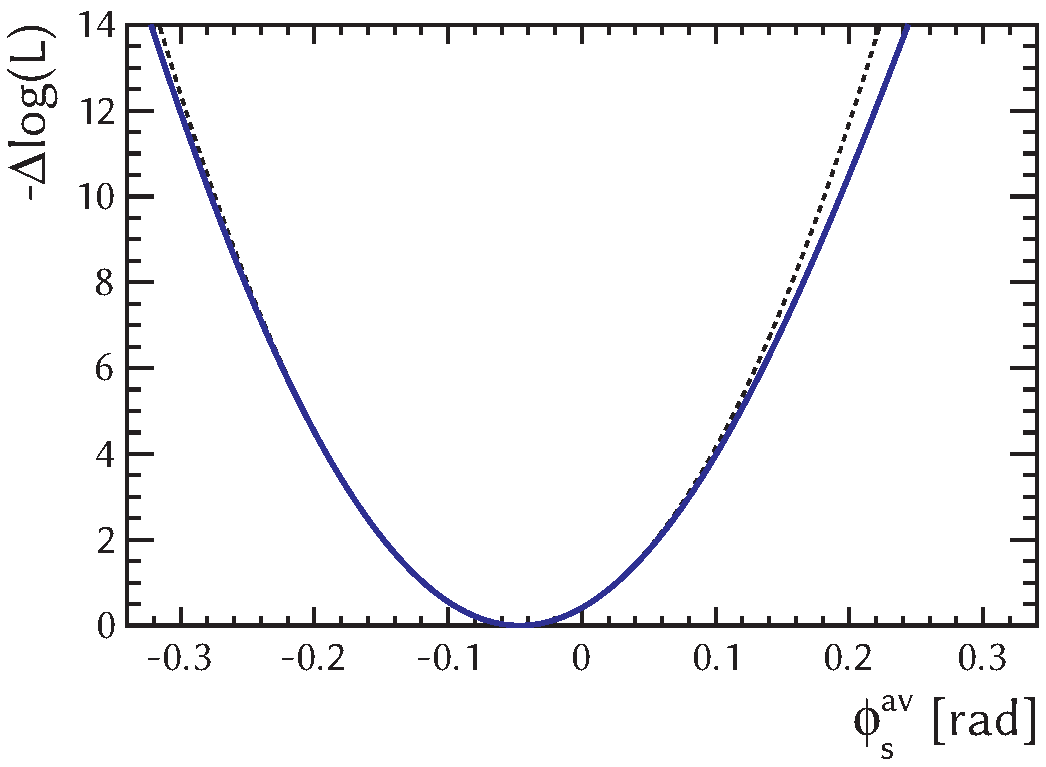
\includegraphics[width=\textwidth]{graphics/results/NLL_polarDep_phiCPAv}
    \caption{}
  \end{subfigure}
  \hfill%
  \begin{subfigure}{0.49\textwidth}
    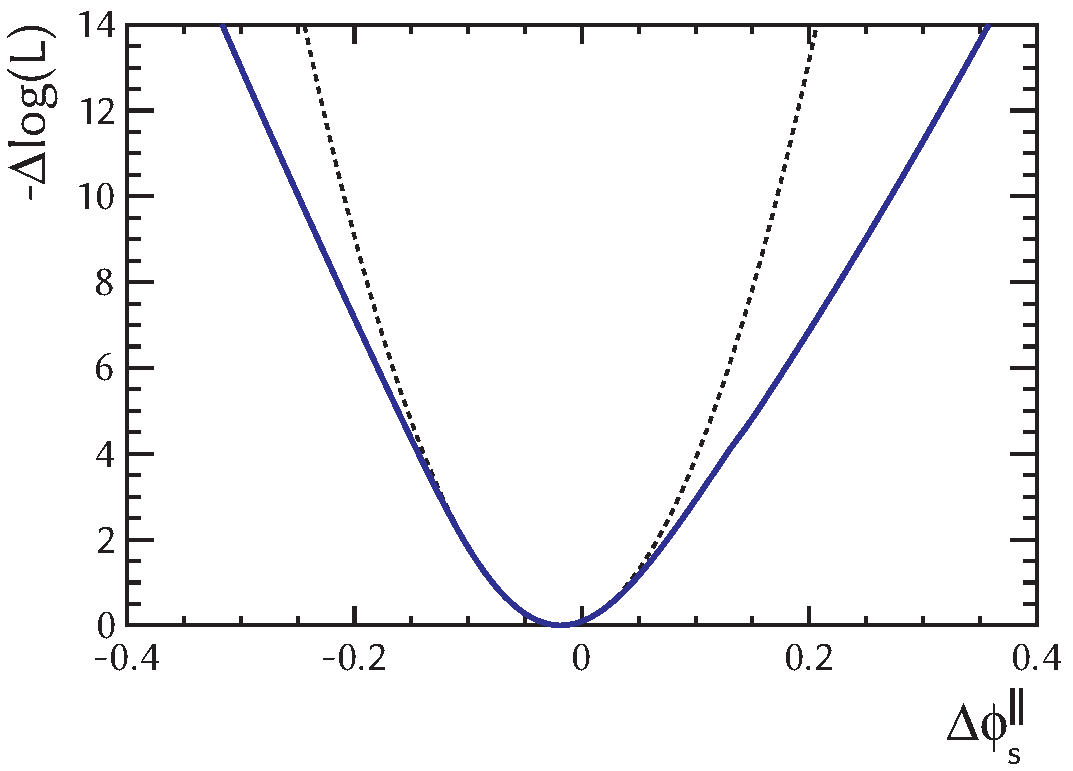
\includegraphics[width=\textwidth]{graphics/results/NLL_polarDep_phiCPRel_Apar}
    \caption{}
  \end{subfigure}

  \vspace*{0.02\textwidth}
  \begin{subfigure}{0.49\textwidth}
    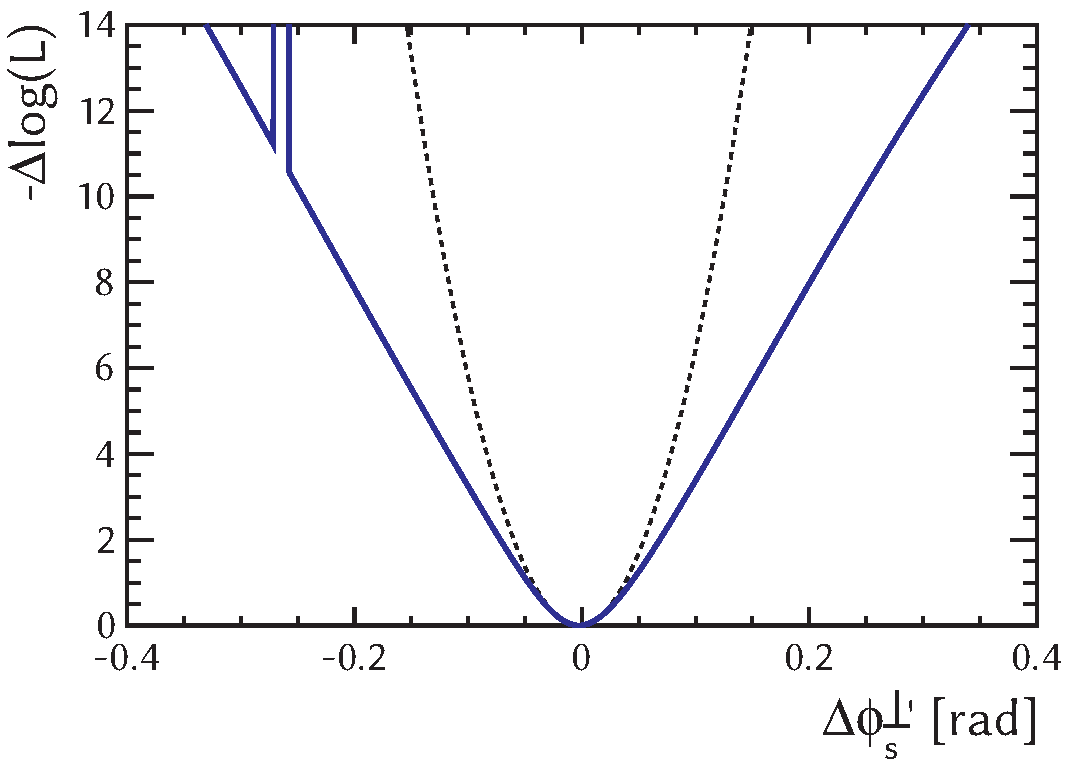
\includegraphics[width=\textwidth]{graphics/results/NLL_polarDep_phiCPRel_AperpApar}
    \caption{}
  \end{subfigure}
  \hfill%
  \begin{subfigure}{0.49\textwidth}
    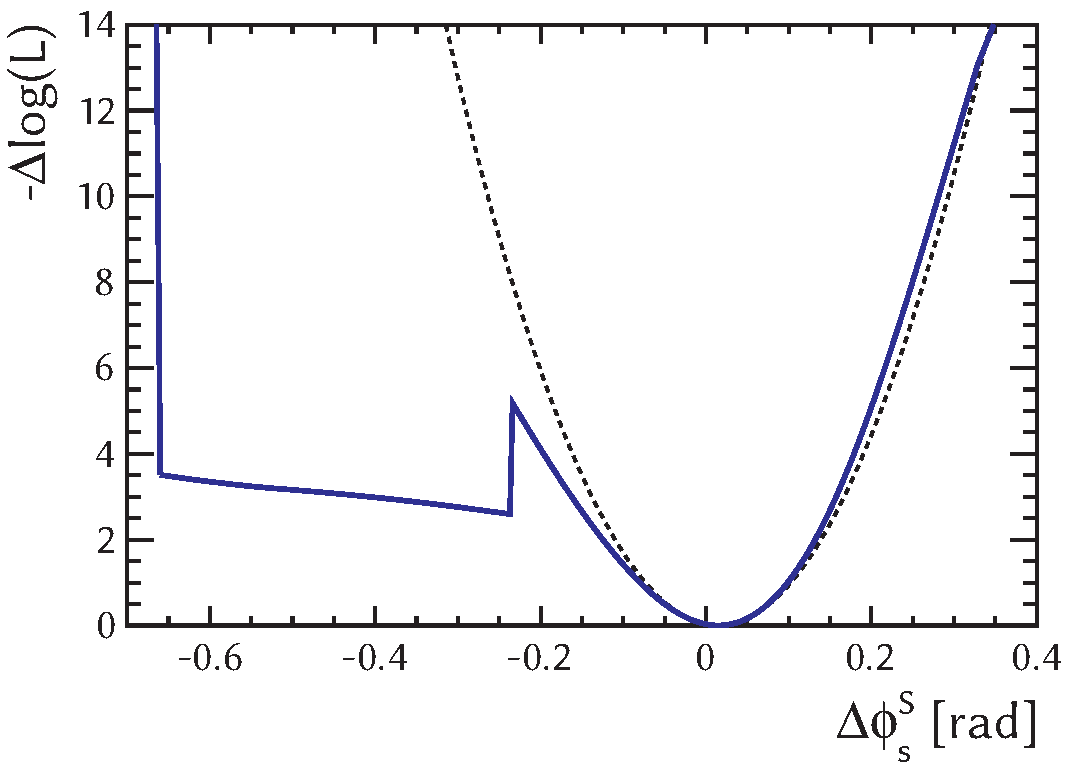
\includegraphics[width=\textwidth]{graphics/results/NLL_polarDep_phiCPRel_AS}
    \caption{}
  \end{subfigure}

  \caption{Log-likelihood scans of the CP-violating phases: (a) $\phisav$, (b) $\Delphispara$, (c) $\Delphisperpp$, and (d) $\DelphisS$.
           See text for details.}
  \label{fig:NLL_CPV_phases}
\end{figure}

\begin{figure}[tbp]
  \centering
  \begin{subfigure}{0.49\textwidth}
    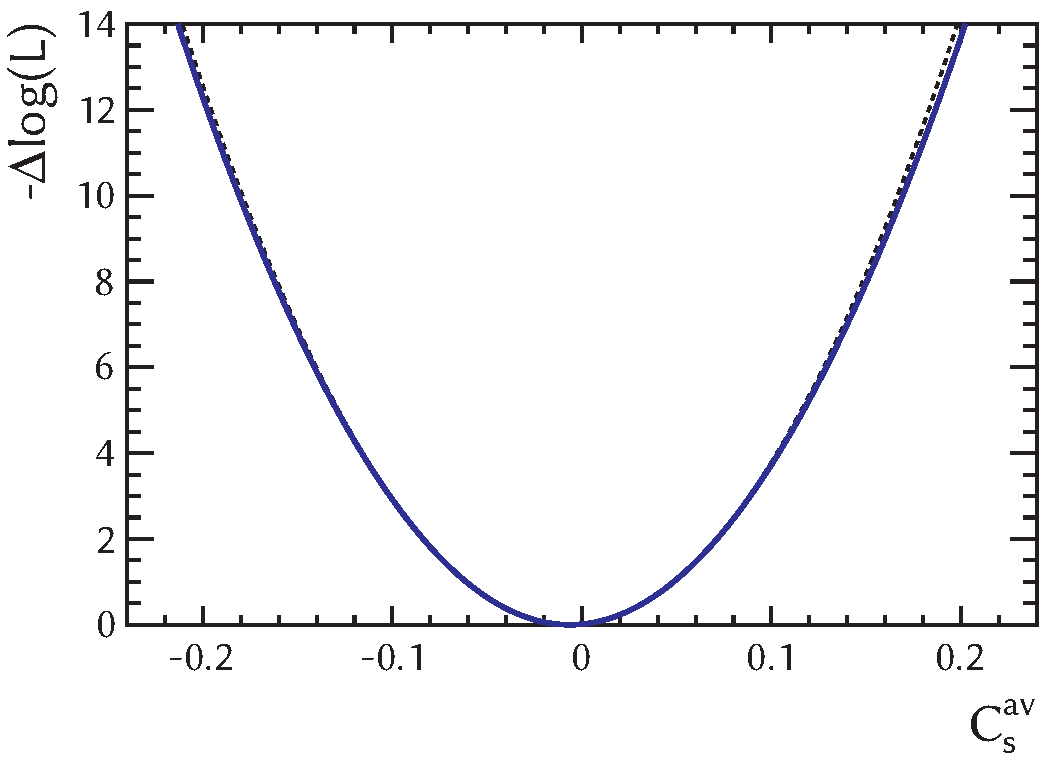
\includegraphics[width=\textwidth]{graphics/results/NLL_polarDep_CCPAv}
    \caption{}
  \end{subfigure}
  \hfill%
  \begin{subfigure}{0.49\textwidth}
    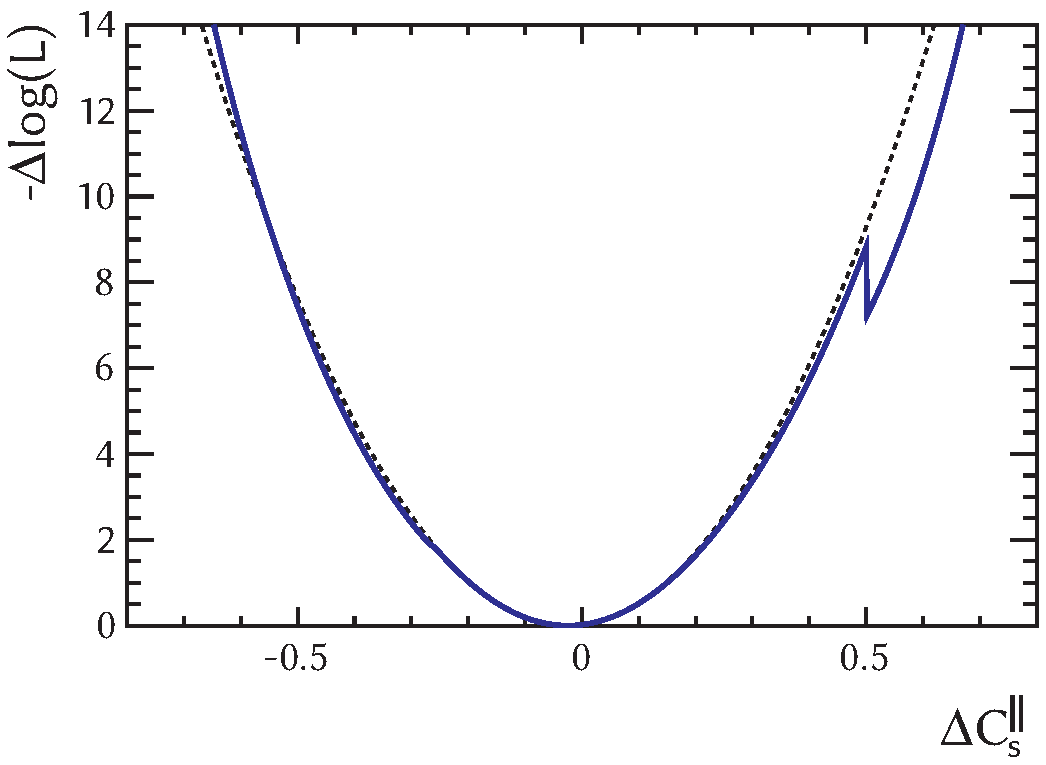
\includegraphics[width=\textwidth]{graphics/results/NLL_polarDep_CCPRel_Apar}
    \caption{}
  \end{subfigure}

  \vspace*{0.02\textwidth}
  \begin{subfigure}{0.49\textwidth}
    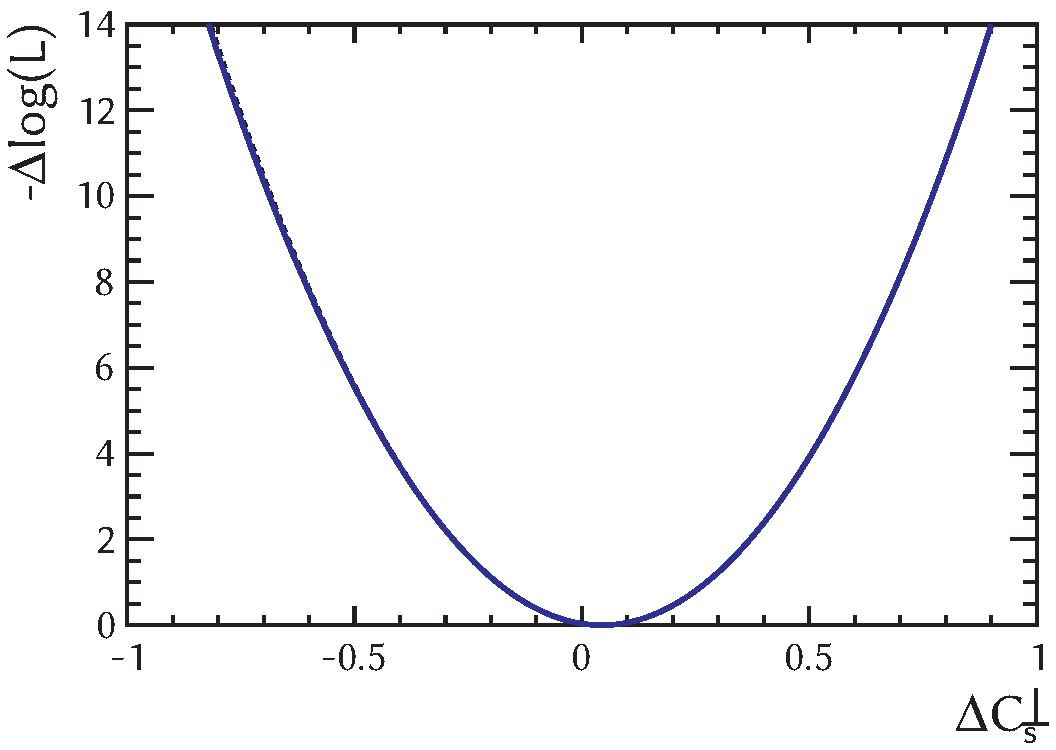
\includegraphics[width=\textwidth]{graphics/results/NLL_polarDep_CCPRel_Aperp}
    \caption{}
  \end{subfigure}
  \hfill%
  \begin{subfigure}{0.49\textwidth}
    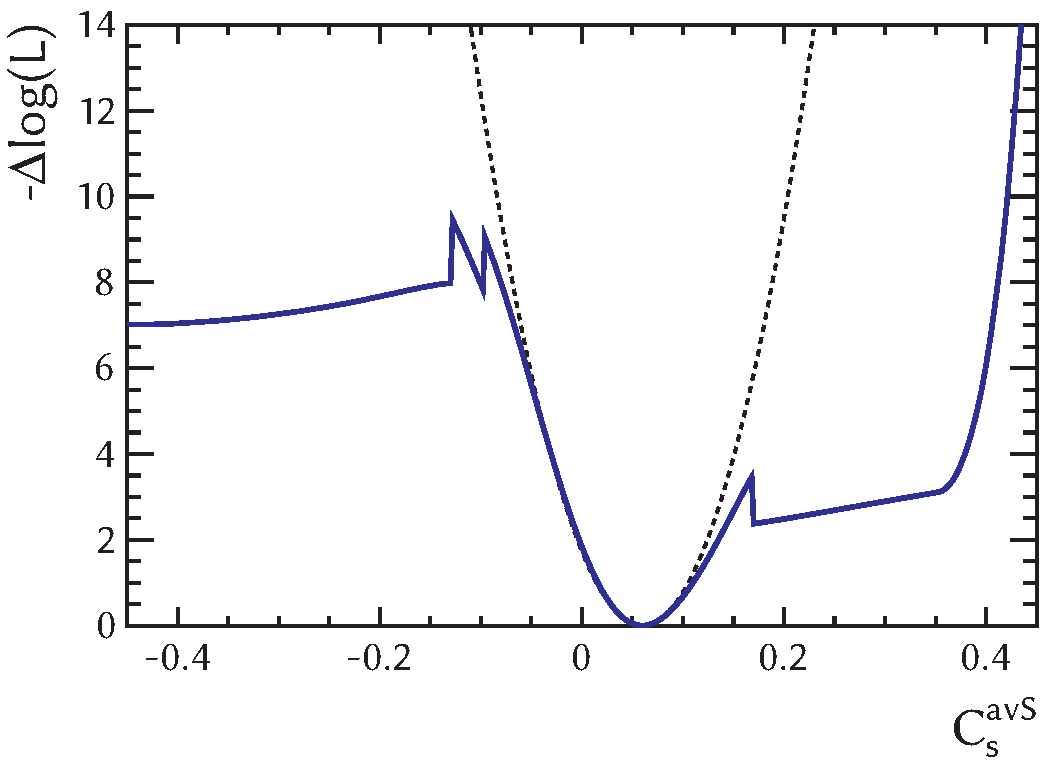
\includegraphics[width=\textwidth]{graphics/results/NLL_polarDep_CCPAv_AS}
    \caption{}
  \end{subfigure}

  \caption{Log-likelihood scans of the asymmetries from CP violation in mixing and in decay:
           (a) $\Csav$, (b) $\DelCspara$, (c) $\DelCsperp$, and (d) $\CsavS$.
           See text for details.}
  \label{fig:NLL_CPV_mixDecay}
\end{figure}

\begin{figure}[tbp]
  \centering
  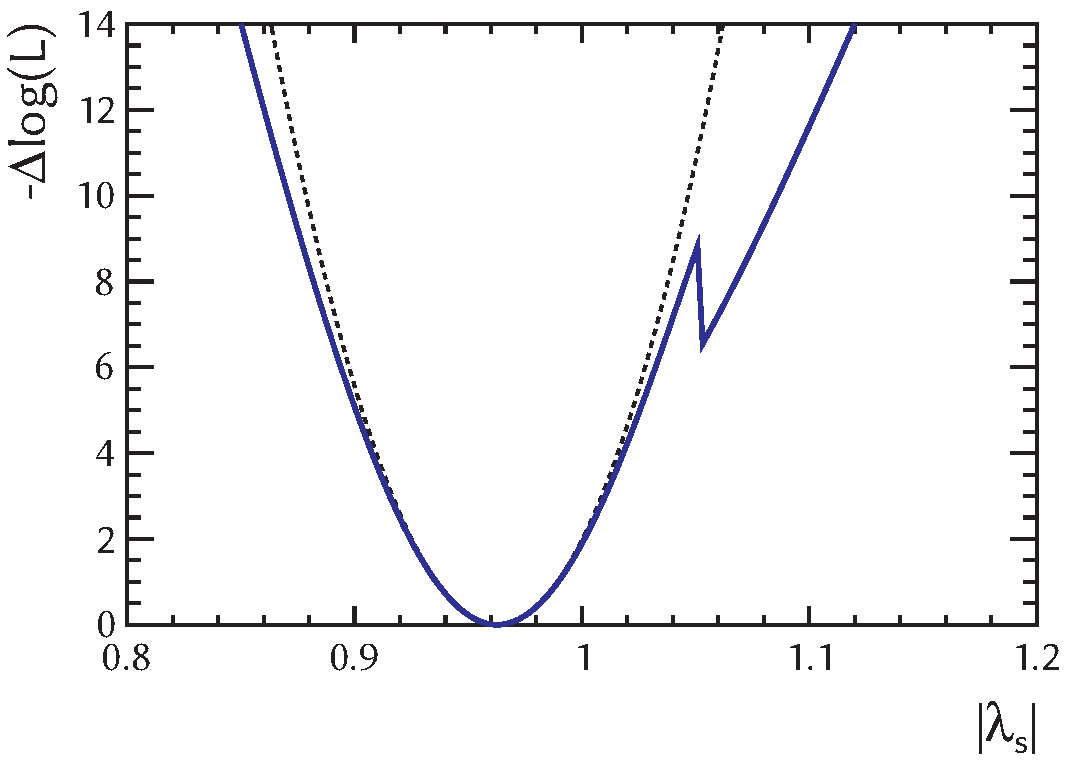
\includegraphics[width=0.49\textwidth]{graphics/results/NLL_lamb_phi_lambdaCP}
  \caption{Log-likelihood scan of $\lamsAbs$. See text for details.}
  \label{fig:NLL_polarDep_lambdas}
\end{figure}

\begin{figure}[tbp]
  \centering
  \begin{subfigure}{0.49\textwidth}
    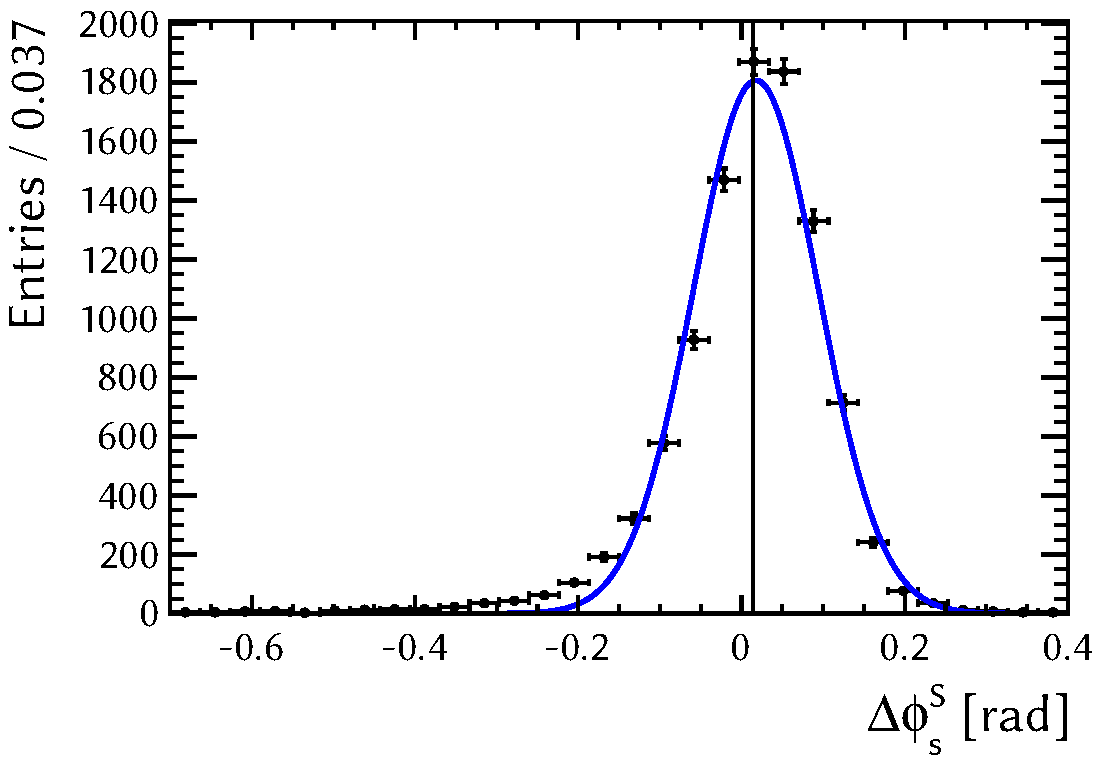
\includegraphics[width=\textwidth]{graphics/results/parDist_polarDep_phiCPRel_AS}
    \caption{}
  \end{subfigure}
  \hfill%
  \begin{subfigure}{0.49\textwidth}
    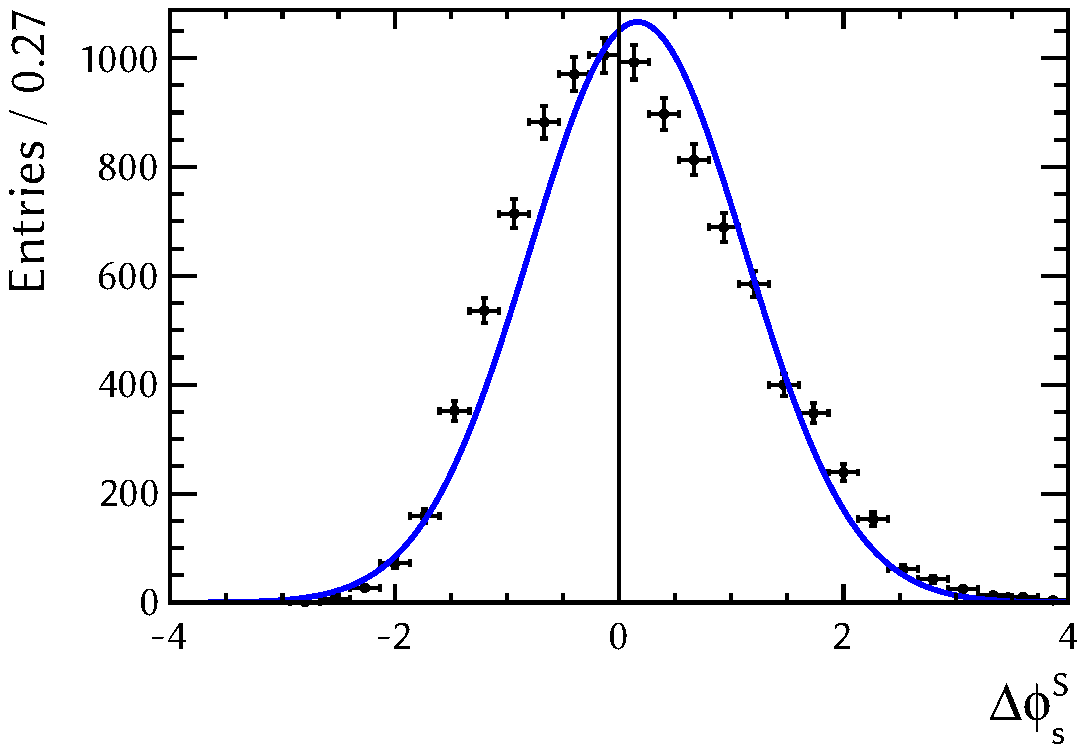
\includegraphics[width=\textwidth]{graphics/results/pullDist_polarDep_phiCPRel_AS}
    \caption{}
  \end{subfigure}

  \vspace*{0.02\textwidth}
  \begin{subfigure}{0.49\textwidth}
    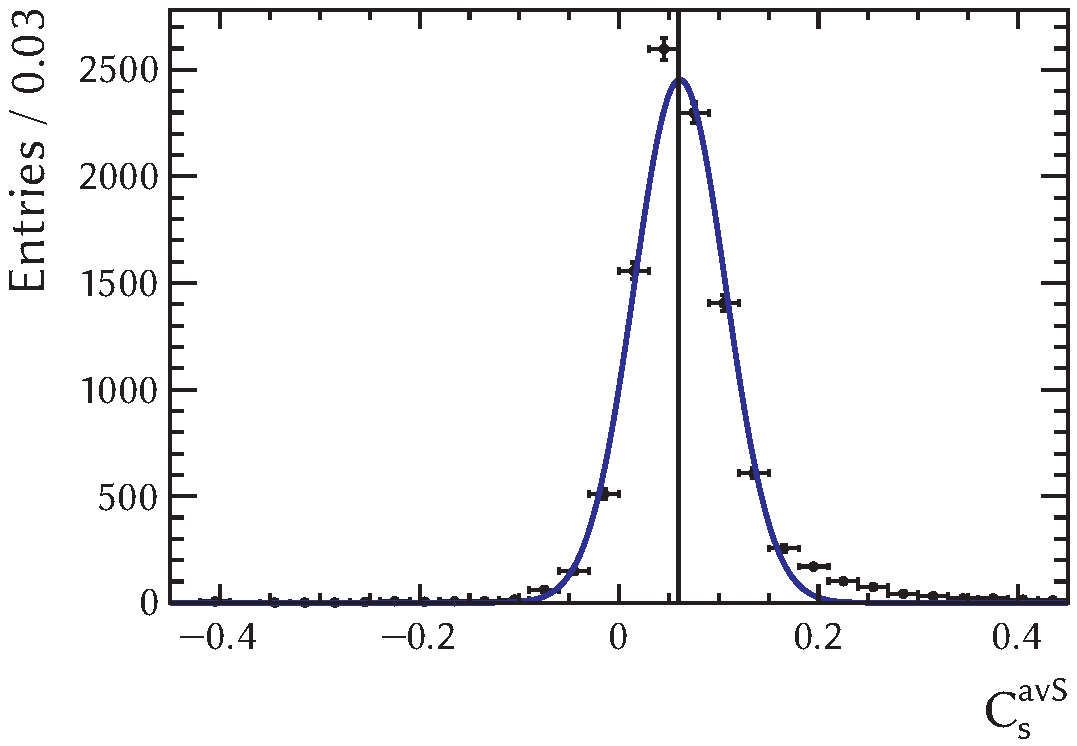
\includegraphics[width=\textwidth]{graphics/results/parDist_polarDep_CCPAv_AS}
    \caption{}
  \end{subfigure}
  \hfill%
  \begin{subfigure}{0.49\textwidth}
    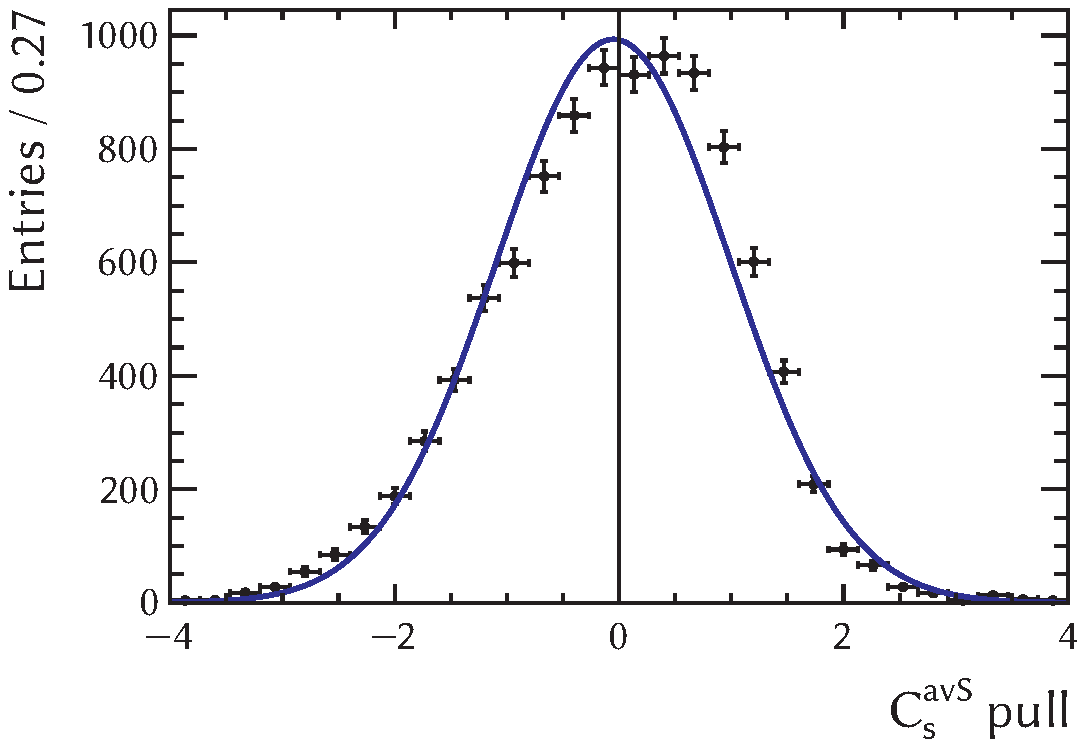
\includegraphics[width=\textwidth]{graphics/results/pullDist_polarDep_CCPAv_AS}
    \caption{}
  \end{subfigure}

  \caption{Distributions of S-wave CP-violation parameters in pseudo experiments:
           (a) $\DelphisS$, (b) $\DelphisS$ pull, (c) $\CsavS$, and (d) $\CsavS$ pull.}
  \label{fig:parDists_SWave_CPV}
\end{figure}

\begin{figure}[tbp]
  \centering
  \begin{subfigure}{0.49\textwidth}
    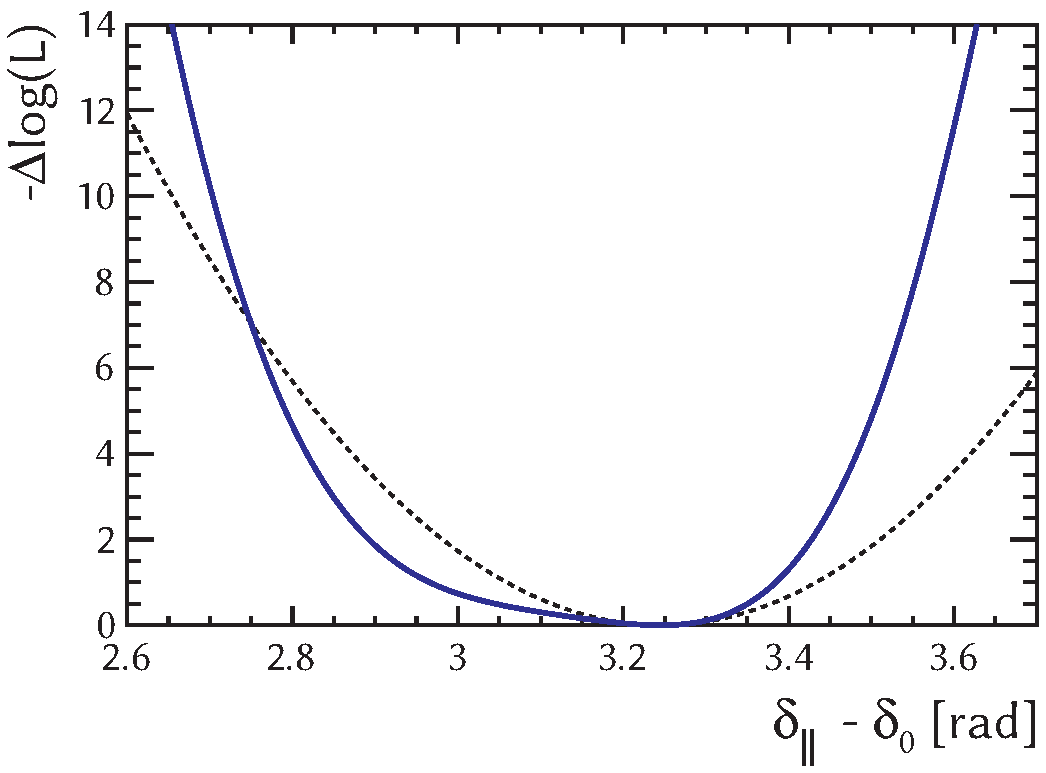
\includegraphics[width=\textwidth]{graphics/results/NLL_polarDep_AparPhase}
    \caption{}
  \end{subfigure}
  \hfill%
  \begin{subfigure}{0.49\textwidth}
    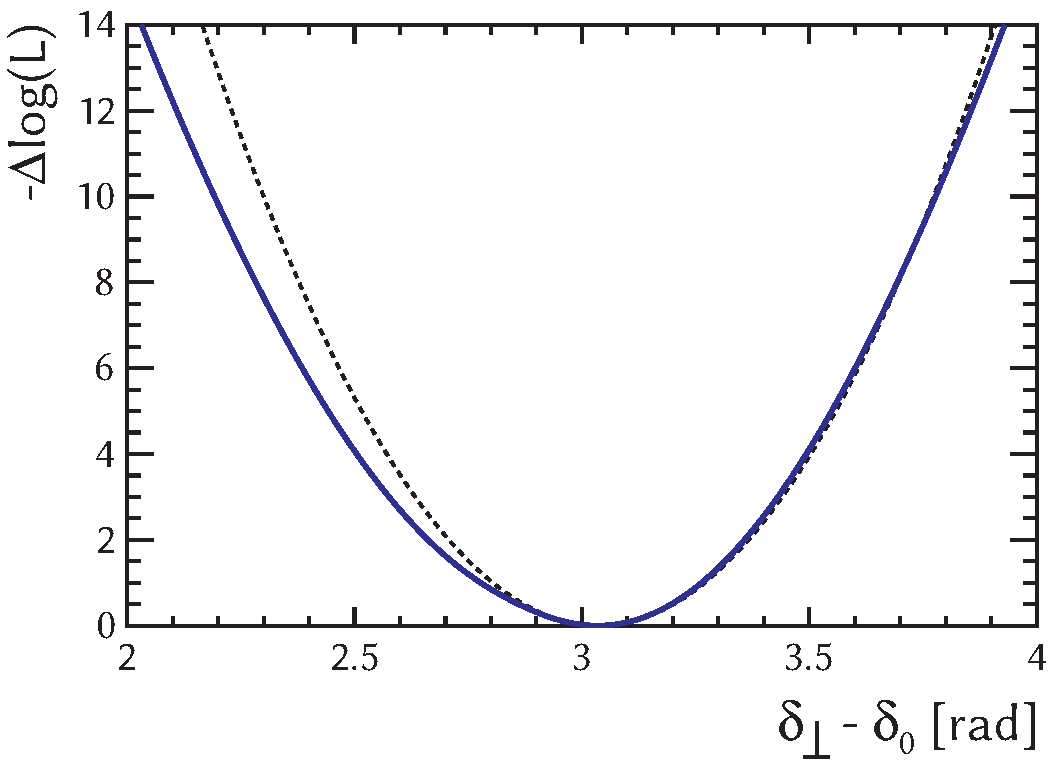
\includegraphics[width=\textwidth]{graphics/results/NLL_polarDep_AperpPhase}
    \caption{}
  \end{subfigure}

  \vspace*{0.02\textwidth}
  \begin{subfigure}{0.55\textwidth}
    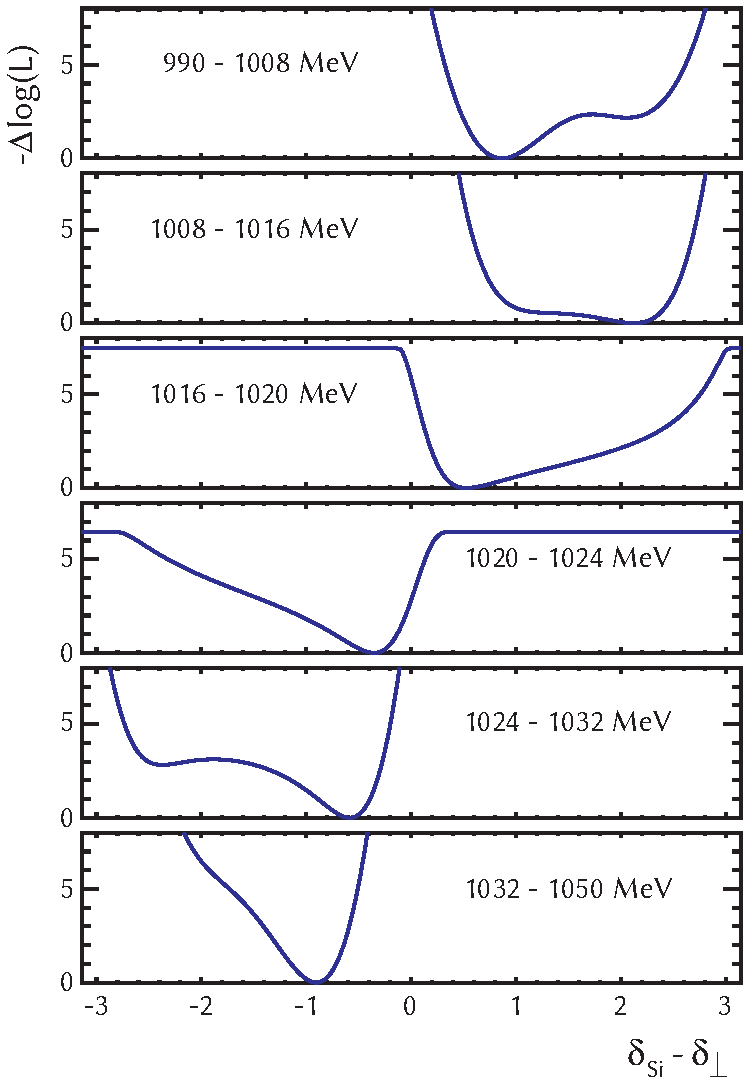
\includegraphics[width=\textwidth]{graphics/results/NLL_polarDep_SWavePhases}
    \caption{}
  \end{subfigure}

  \caption{Log-likelihood scans of the phases of the transversity amplitudes (likelihood with polarization-dependent CP violation):
           (a) $\delparzero$, (b) $\delperpzero$,
           (c) $\delSperp[i]$, where the $\KK$-mass bin is indicated with the corresponding $\KK$-mass range.
           See text for details.}
  \label{fig:NLL_polarDep_transPhases}
\end{figure}

\begin{figure}[tbp]
  \centering
  \begin{subfigure}{0.49\textwidth}
    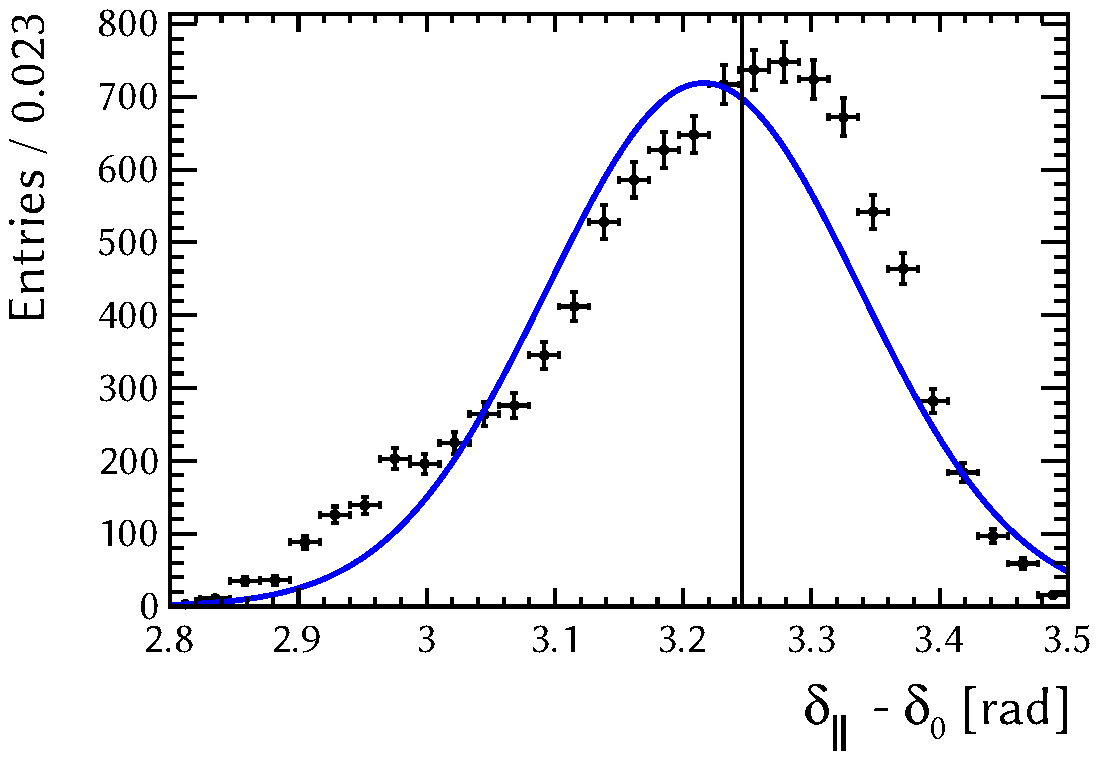
\includegraphics[width=\textwidth]{graphics/results/parDist_polarDep_AparPhase}
    \caption{}
  \end{subfigure}
  \hfill%
  \begin{subfigure}{0.49\textwidth}
    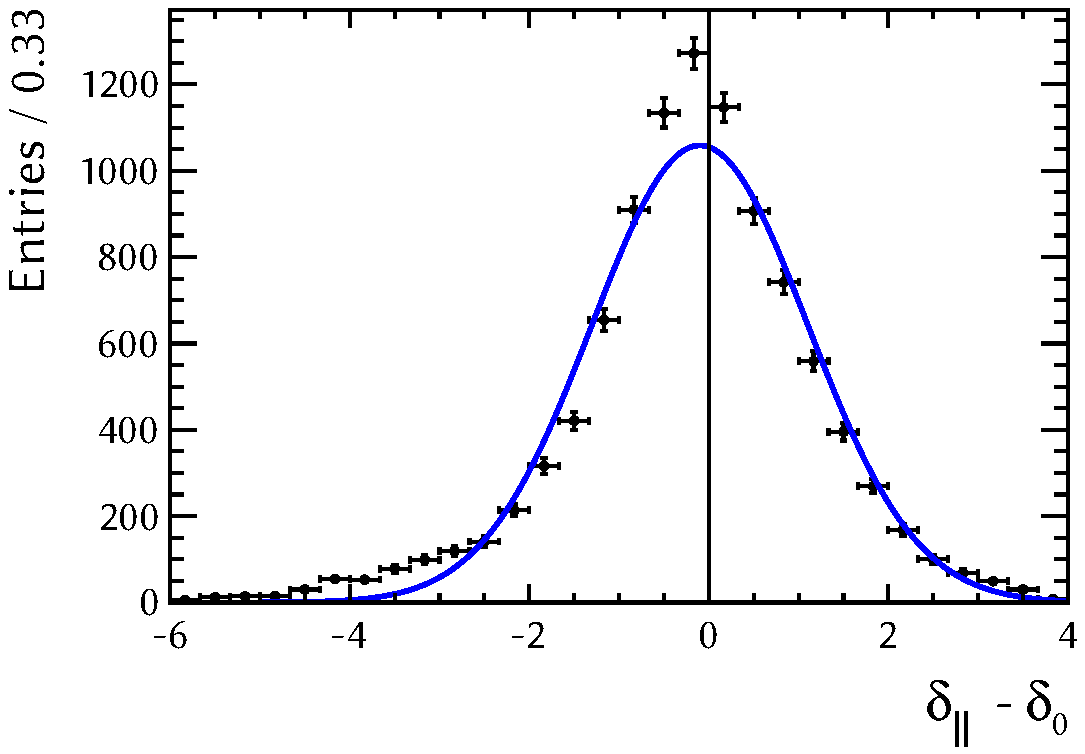
\includegraphics[width=\textwidth]{graphics/results/pullDist_polarDep_AparPhase}
    \caption{}
  \end{subfigure}

  \vspace*{0.02\textwidth}
  \begin{subfigure}{0.49\textwidth}
    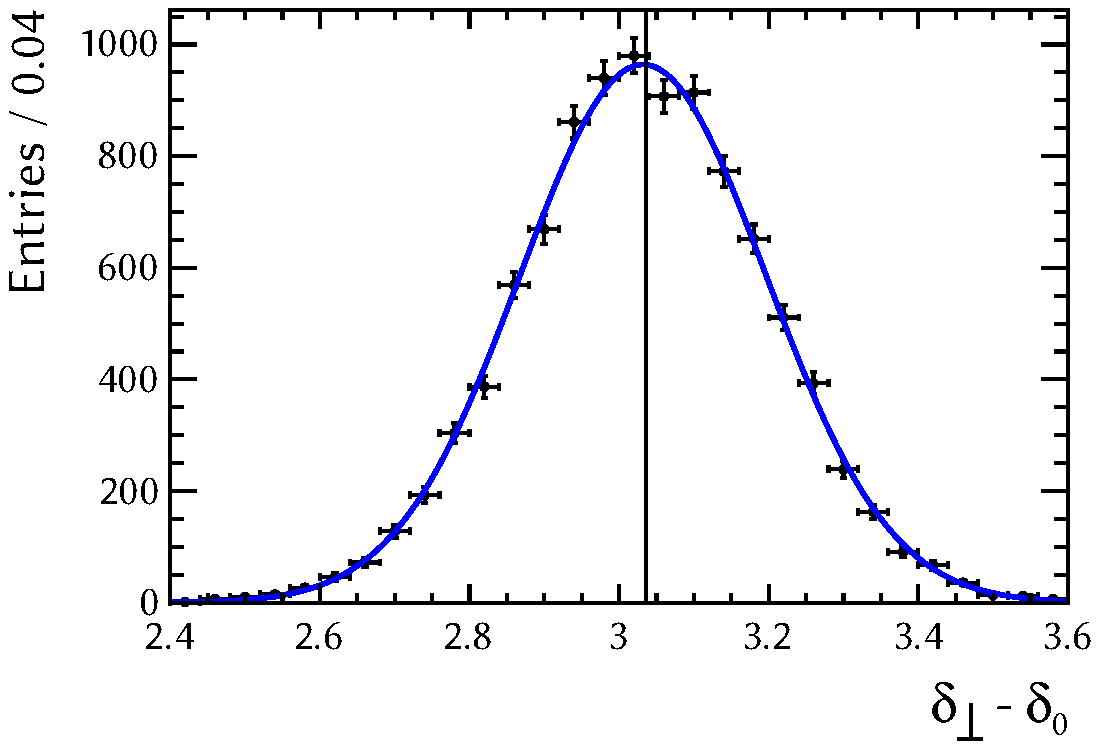
\includegraphics[width=\textwidth]{graphics/results/parDist_polarDep_AperpPhase}
    \caption{}
  \end{subfigure}
  \hfill%
  \begin{subfigure}{0.49\textwidth}
    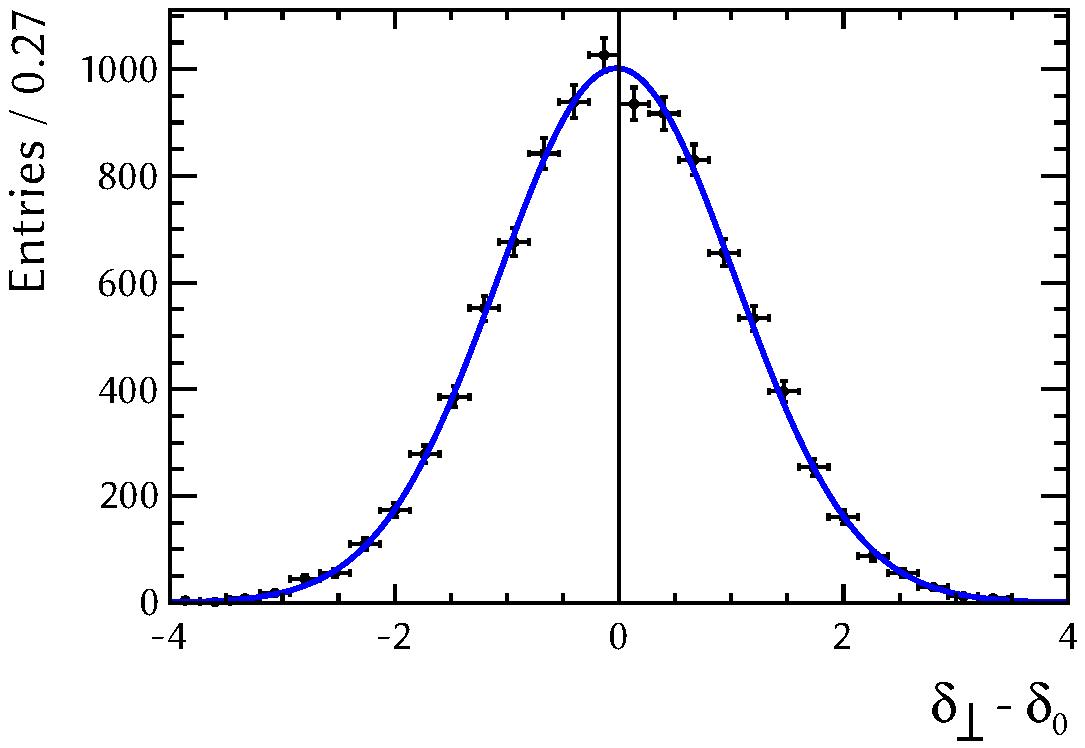
\includegraphics[width=\textwidth]{graphics/results/pullDist_polarDep_AperpPhase}
    \caption{}
  \end{subfigure}

  \caption{Distributions of the phases of the transversity amplitudes (maximum of the likelihood with polarization-dependent CP violation)
           in pseudo experiments:
           (a) $\delparzero$, (b) $\delparzero$ pull, (c) $\delperpzero$, and (d) $\delperpzero$ pull.}
  \label{fig:parDists_parperpPhases}
\end{figure}

\begin{figure}[tbp]
  \centering
  \begin{subfigure}{0.49\textwidth}
    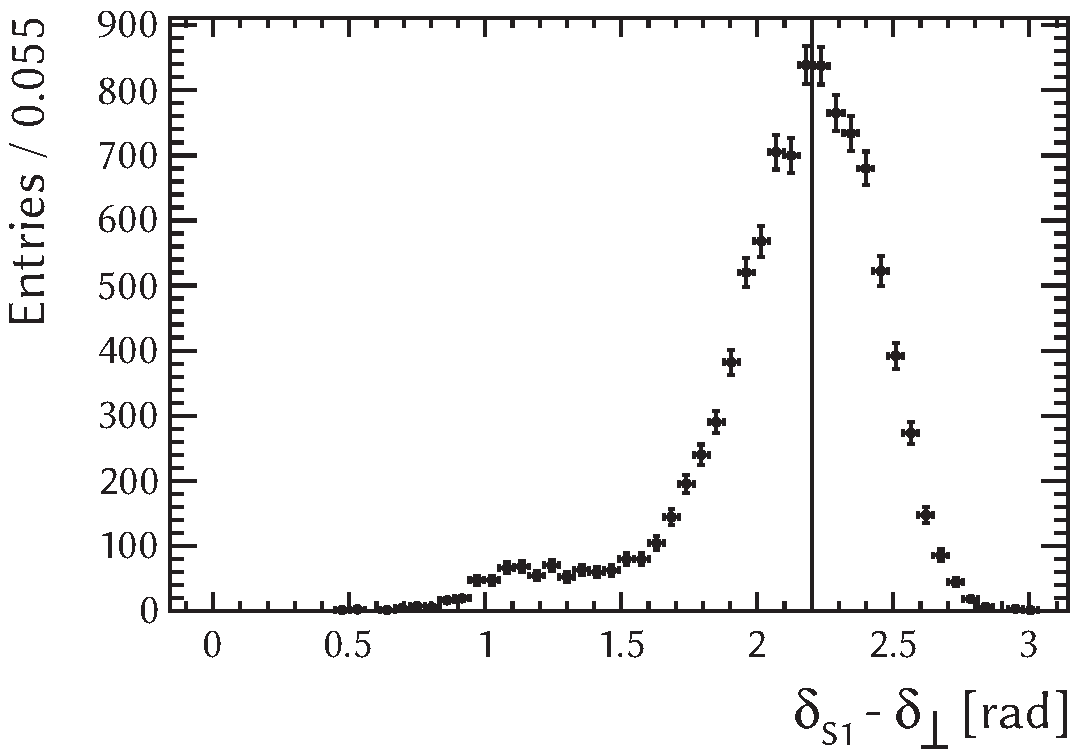
\includegraphics[width=\textwidth]{graphics/results/parDist_polarDep_ASOddPhase_bin0}
    \caption{}
  \end{subfigure}
  \hfill%
  \begin{subfigure}{0.49\textwidth}
    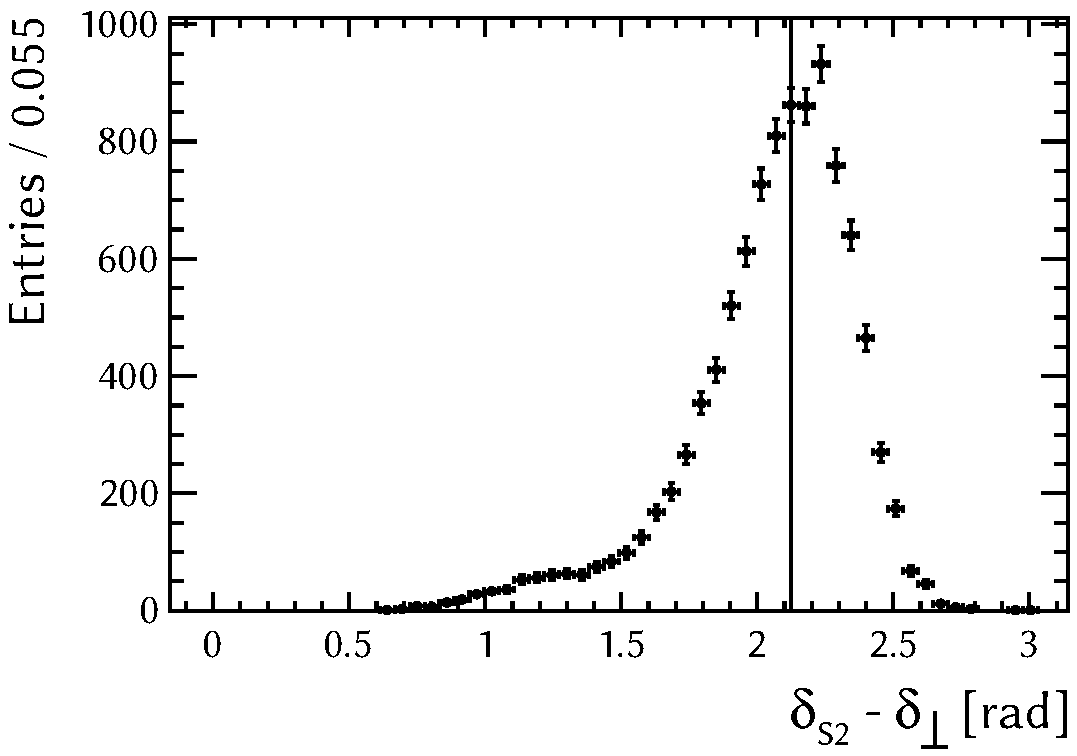
\includegraphics[width=\textwidth]{graphics/results/parDist_polarDep_ASOddPhase_bin1}
    \caption{}
  \end{subfigure}

  \vspace*{0.02\textwidth}
  \begin{subfigure}{0.49\textwidth}
    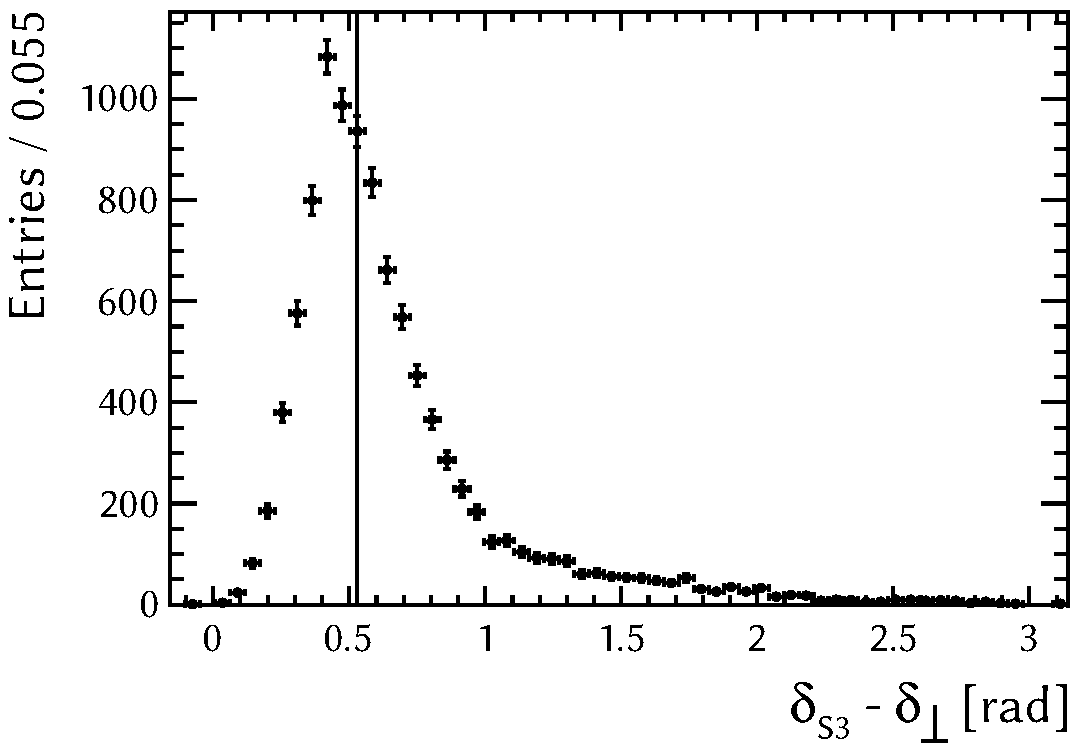
\includegraphics[width=\textwidth]{graphics/results/parDist_polarDep_ASOddPhase_bin2}
    \caption{}
  \end{subfigure}
  \hfill%
  \begin{subfigure}{0.49\textwidth}
    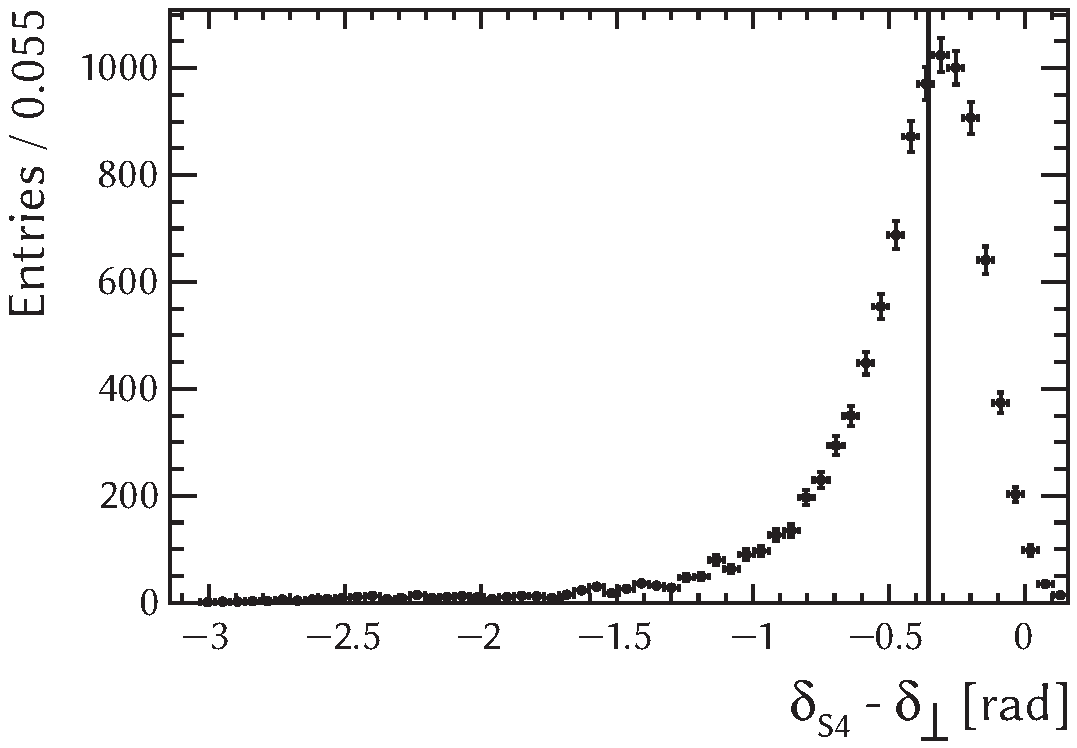
\includegraphics[width=\textwidth]{graphics/results/parDist_polarDep_ASOddPhase_bin3}
    \caption{}
  \end{subfigure}

  \vspace*{0.02\textwidth}
  \begin{subfigure}{0.49\textwidth}
    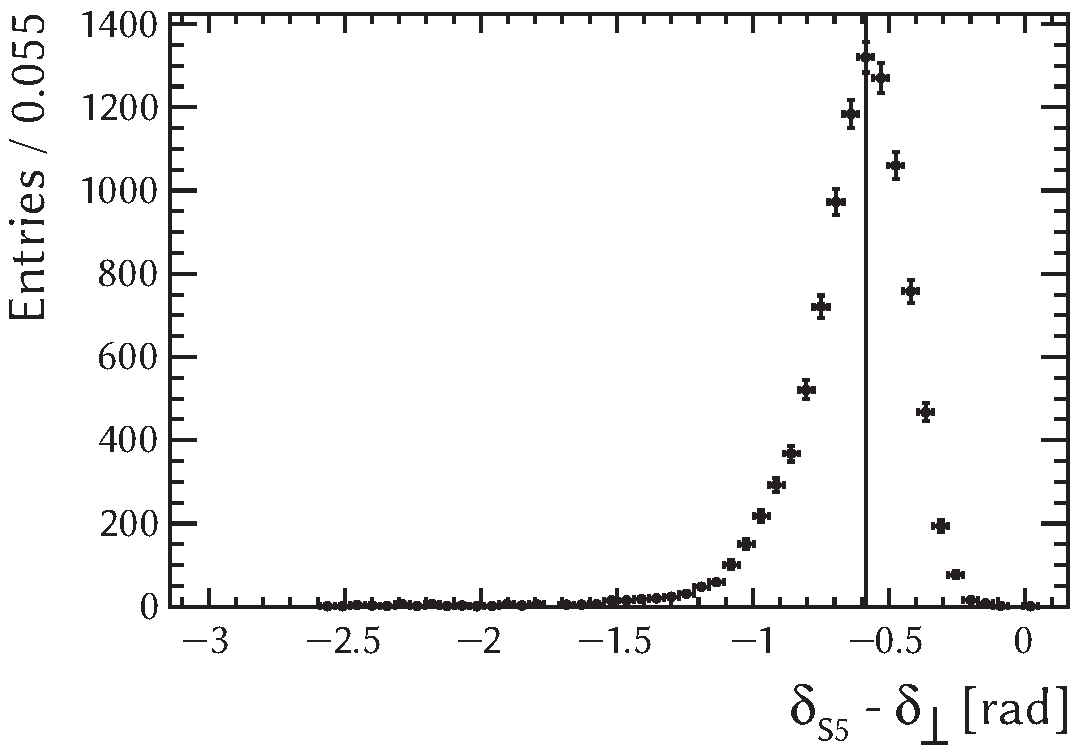
\includegraphics[width=\textwidth]{graphics/results/parDist_polarDep_ASOddPhase_bin4}
    \caption{}
  \end{subfigure}
  \hfill%
  \begin{subfigure}{0.49\textwidth}
    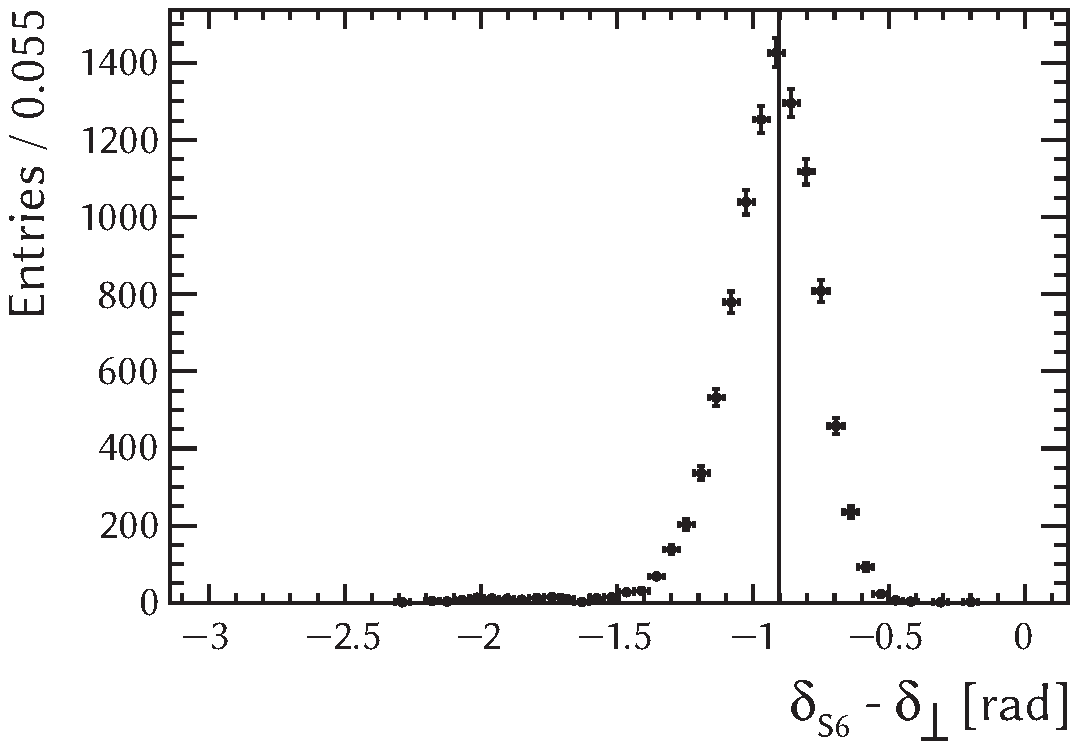
\includegraphics[width=\textwidth]{graphics/results/parDist_polarDep_ASOddPhase_bin5}
    \caption{}
  \end{subfigure}

  \caption{Distributions of the phases of the S-wave amplitudes (maximum of the likelihood with polarization-dependent CP violation)
           in pseudo experiments in the six $\KK$-mass bins:
           (a) 990--1008\unitsp\MeV, (b) 1008--1016\unitsp\MeV, (c) 1016--1020\unitsp\MeV,
           (d) 1020--1024\unitsp\MeV, (c) 1024--1032\unitsp\MeV, and (f) 1032--1050\unitsp\MeV.}
  \label{fig:parDists_SWavePhases}
\end{figure}

